\chapter {Establishing Benchmark of Physics-based PMP Estimation using A Hybrid Approach}
\label{ch:WRR}

\externaldocument{appendixWRR}

This chapter has been published mostly in its current form in the \textit{Water Resources Research}. \textcopyright Chen and Hossain. Used with permission.\\

\bigbreak

\noindent
\hangafter=1
\setlength{\hangindent}{2em}
Chen, X., Hossain, F., and Leung, R. L., Probable maximum precipitation in the U.S. Pacific Northwest in a changing climate. \textit{Water Resources Research} (under review).

\vspace{10mm}

\noindent
\textit{\textbf{Abstract}}
 
The safety of large and aging water infrastructures is gaining attention in water management given the accelerated rate of change in landscape, climate and society. In current engineering practice, such safety is ensured by the design of infrastructure for the Probable Maximum Precipitation (PMP). Recently, several numerical modeling approaches have been proposed to modernize the conventional and ad hoc PMP estimation approach. However, the underlying physics have not been investigated and thus differing PMP estimates are obtained without clarity on their interpretation. In this study, we present a hybrid approach that takes advantage of both traditional engineering practice and modern climate science to estimate PMP for current and future climate conditions. The traditional PMP approach is improved and applied to five statistically downscaled CMIP5 model outputs, producing an ensemble of PMP estimates in the Pacific Northwest (PNW) during the historical (1970-2016) and future (2050-2099) time periods. The new historical PMP estimates are verified against the traditional estimates. PMP in the PNW will increase by $50\%\pm30\%$ of the current level by 2099 under the RCP8.5 scenario. Most of the increase is caused by warming, which mainly affects moisture availability through increased sea surface temperature, with minor contributions from changes in storm efficiency in the future. Moist track change tends to reduce the future PMP. Compared with extreme precipitation, PMP exhibits higher internal variability. Thus long-time records of high-quality data in both precipitation and related meteorological fields (temperature, wind fields) are required to reduce uncertainties in the ensemble PMP estimates.

\vspace{20mm}

\section{Introduction}

In the past century, numerous water infrastructures have been built to facilitate irrigation, hydropower generation, transportation and municipal water use. In a changing climate, extreme precipitation events are projected to be more frequent and intense, exceeding known historical records [\textit{Trenberth et al.}, 2003; \textit{Allan and Soden}, 2008; \textit{Kunkel et al.}, 2013a]. Along with structural safety, the hydrologic safety of water infrastructures is therefore gaining more attention, since overtopping or embankment failure would bring catastrophic human and societal loss [\textit{Evans et al.}, 2000; \textit{Casagli et al.}, 2006; \textit{Lane}, 2013]. For example, the structural damage to both the primary and the emergency spillways of the Oroville Dam in California, which could have been exacerbated by hydrologic failure, during a series of heavy rainstorms in February 2017 led to an evacuation of over 188,000 downstream residents [\textit{Vahedifard et al.}, 2017].

Most of the water infrastructures, especially the hazardous ones located upstream of population centers, are often designed considering the standard Probable Maximum Precipitation (PMP) [\textit{Hossain et al.}, 2012]. PMP, by its definition, is the theoretical maximum precipitation that a given watershed can receive in a given duration of time [\textit{World Meteorological Organization (WMO)}, 1986]. WMO suggests several methods for PMP estimation: statistical method, generalized method, transposition method, and moisture maximization method [\textit{Hershfield}, 1965; \textit{Rakhecha and Kennedy}, 1985; \textit{World Meteorological Organization (WMO)}, 1986; \textit{Rakhecha and Singh}, 2009]. The moisture maximization approach is the recommended method in the US. NOAA has published a series of Hydro-Meteorological Reports (HMRs) that provide instructions for PMP estimation in various climatological regions across the US [\textit{Schreiner and Riedel}, 1978]. The moisture maximization method estimates PMP as $PMP=P\times{PW_m}/PW$, where $P$ is the observed precipitation, $PW$ is the observed precipitable water, and $PW_m$ is the climatologically maximum precipitable water (estimated from surface dew point temperature assuming hydrostatic conditions).

The moisture maximization method has been criticized in several studies as being insufficiently grounded in physics [\textit{Abbs}, 1999]. Also, the accuracy of this approach heavily relies on availability and quality of observation data, which makes PMP estimation less reliable in regions where sufficient observation has not been obtained. Traditionally, PMP is treated as a static value, estimated using long-term precipitation and related meteorological data (such as humidity, temperature, winds). The static nature of PMP estimation has been questioned as global warming can lead to more intense precipitation. Non-stationary analyses of extreme precipitation also suggest that PMP, an upper bound of extreme precipitation, is likely to change in the future [\textit{Cheng and AghaKouchak}, 2014; \textit{Cheng et al.}, 2014; \textit{Gao et al.}, 2016; \textit{Wi et al.}, 2016].

In recent years, two significant advancements have been made to modernize PMP estimation used in engineering practice. One of them is the ability to derive uncertainty associated with PMP estimation [\textit{Salas et al.}, 2014; \textit{Micovic et al.}, 2015]. Another advancement is the introduction of numerical atmospheric models to enable a more physics-based estimation of PMP [\textit{Tan}, 2010; \textit{Ohara et al.}, 2011; \textit{Ishida et al.}, 2015; C\textit{hen and Hossain}, 2016; \textit{Chen et al.}, 2017]. In atmospheric model-based estimates, PMP is obtained by modifying the initial/boundary conditions of extreme precipitation event simulations, such as increased moisture availability (usually by setting relative humidity RH to 100\%), increased air temperature, spatially shifted initial/boundary conditions, or artificially generated convergent wind fields. Most studies focused on the reconstruction of PMP from various reanalysis data, although climate model data have also been explored [\textit{Tan}, 2010; \textit{Ohara et al.}, 2011; \textit{Beauchamp et al.}, 2013; \textit{Rousseau et al.}, 2014; \textit{Rouhani and Leconte}, 2016; \textit{Lee et al.}, 2017; \textit{Rastogi et al.}, 2017]. These studies suggest that carefully selected climate data, such as the CMIP5 data, may have value for historical PMP estimation. However, care should be taken in selecting climate models, as climate simulations (such as CMIP5) exhibit a wide range of precipitation estimation [\textit{Sheffield et al.}, 2013]. Alternatively, regional climate model output can be used for PMP estimation with the advantage of providing more spatially resolved precipitation features. These studies reveal the potential of climate projections to quantify the sensitivity of PMP to climate change [\textit{Beauchamp et al.}, 2013; \textit{Rousseau et al.}, 2014; \textit{Rastogi et al.}, 2017].

Up to now, such model-based approaches have not been widely validated, and their physical basis has not been thoroughly established. By modifying different variables in the simulations, the modeling approaches implicitly assume that extreme precipitation will be more sensitive to the variables modified. For example, the RH maximization approach assumes that storm magnitude is more sensitive to the RH level, while a wind perturbation approach assumes that storm is more sensitive to the moisture convergence. Several other approaches, such as the spatial shift of initial/boundary conditions [\textit{Ohara et al.}, 2011; \textit{Ishida et al.}, 2015], produce results that are even harder to interpret. From the modelling perspective, moving the atmospheric boundary condition spatially induces a shift in the land surface condition. In regions where surface heterogeneity is an important driver of precipitation variability, shifting the atmospheric boundary condition can result in drastic changes in the storm characteristics and hence PMP estimation.

The aforementioned approaches have not been comprehensively compared to the traditional estimates up to now, and the PMP estimation results often differ from traditional values that have been used in the infrastructure design stage. Such inconsistency makes it hard to use the new results to reevaluate the safety of infrastructures. Lastly, most of the modelling studies focused on selected watersheds, making it harder to derive general guidelines for engineering designing across regions (an exception is the study by \textit{Rastogi et al.} [2017], which focused on building the area-duration-intensity curves).

The traditional engineering approach takes all the information from historical observations, while an atmospheric model-based physical approach accounts for all dynamical and physical processes that influence the storms. Due to a significant gap between these two contrasting approaches, it is hard for the respective communities (i.e., engineering for conventional PMP and scientists for model-based PMP) to communicate the needs and constraints for collaborative advancements. This is especially important when evaluating the sensitivity of PMP to climate change since the reference (i.e., historical PMP) has been estimated quite differently. Therefore, it is important to bridge the gap between the two contrasting types of estimation. In this study, a hybrid approach of applying the traditional methodology to climate model outputs is proposed. Climate model outputs provide long-term records of extreme events, which would improve estimates of extreme events and help reveal the climatic trend of PMP estimate. The non-stationary issues can therefore be addressed by estimating PMP using future climate projections. Most importantly, the availability of ensemble climate model output (e.g., ~30 models used in IPCC AR5) allows derivation of ensemble PMP estimates useful for evaluating the statistical significance of future changes in PMP. An added benefit of the hybrid approach is the ease of use by those who are already familiar with the conventional approach used in the current engineering practice. No complex and computationally intensive modeling resources are required in our proposed approach as model outputs are readily available from the climate modeling community.

In this chapter, the hybrid approach is used to reconstruct the PMP in the Pacific Northwest region and investigate the likely future change in PMP under projected climate change by climate models. Our research questions are:

(1) What are the PMP estimates in the US PNW region based on climate science and current engineering convention?

(2) How will such PMP estimates change in the future in the PNW region and what are the contributions of various climate factors to the PMP change?

\section{Data and methods}

In this study, we focus on the Pacific Northwest, as shown in Figure \ref{fig:5-1}. Panel \ref{fig:5-1}a shows the topography from ETOPO1 database [\textit{Amante and Eakins}, 2009] in the study domain, which features the Cascade Range along the coast. Extreme precipitation in this region is mainly triggered by atmospheric river events that transport significant atmospheric moisture from the Pacific Ocean [\textit{Leung and Qian}, 2009; \textit{Dettinger}, 2011; \textit{Neiman et al.}, 2011; \textit{Ralph et al.}, 2011]. As storms approach from the Pacific Ocean, extreme precipitation in this region shows a distinctive signature across the Cascade Range as abundant moisture condenses and is converted to precipitation when air mass is lifted over the mountain, so precipitation is much stronger on the west or windward side of the Range. Figure \ref{fig:5-1} shows the PMP estimation from this study for each Hydrological Unit (HU) in Pacific Northwest. HU is developed by US Geological Survey (USGS) to define various hydrological characteristics such as lakes, watersheds or catchments [\textit{Seaber et al.}, 1987]. The red dots denote the locations of dams/reservoirs where PMP estimations are available in HMR57 (HMR for Pacific Northwest region). These values were later used to evaluate the PMP estimations from this study.

\begin{figure}[htbp]
	\includegraphics[width=\linewidth]{pics/ch5/fig1.jpg}
	\caption{Pacific Northwest (PNW) domain in the study. Panel (a) illustrates the surface elevation in the PNW study domain. Panel (b) highlights all the hydrological unit (HU) basins in the PNW. The colors show the hybrid PMP estimation from this study. The red dots denote locations where PMP estimation is available in Hydrometeorological Report No. 57 (HMR57). These HMR57 PMP values are shown in Figure \ref{fig:5-5}.}
	\label{fig:5-1}
\end{figure}

Our hybrid PMP estimation uses five CMIP5 model results for PMP estimation, and in total ten CMIP5 models are used for robust uncertainty estimation [\textit{Mote et al.}, 2011]. The PMP estimation approach follows the HMR57 instructions. Necessary modifications are made to adapt climate model data and the trajectory procedure that is modernized using the HYSPLIT (Hybrid Single-Particle Lagrangian Integrated Trajectory) model. Details about the data and the method are presented below. We chose 1970-2016 as the historical PMP study period and 2050-2099 RCP8.5 scenario as the future PMP study period.

\subsection{CMIP5 climate model data}

Five CMIP5 models are used for ensemble estimation of PMP, and an additional  five models are also used to estimate the uncertainty range of PMP estimation. Their information is summarized in Table \ref{table:5-1}. These ten models were selected from the comprehensive evaluation of CMIP5 models over the PNW region using multiple metrics [\textit{Rupp et al.}, 2013], and they cover a wide range of model performance from best to average. The five models used in PMP estimation were selected based on their performance in capturing the statistics of atmospheric river frequency [\textit{Gao et al.}, 2015]. This selection is discussed in detail in the results section. These five models also cover a range of model resolution (between $0.75^{\circ}$ and $2^{\circ}$), so the impact of climate model resolution on the PMP estimation can also be evaluated.

\begin{sidewaystable}[htbp]
	\centering
	\caption{Information of the 10 selected CMIP5 models used in this chapter}
	\begin{threeparttable}
		\begin{tabular}{cccc}
			\hline
			\multirow{2}{*}{Model} & \multirow{2}{*}{Modeling center} & Horizontal grid size & Number of vertical\\
			                       &                                  & (atmospheric)        & layers \\
			\hline
			            & Commonwealth Scientific and Industrial Research                &                           &    \\
			ACCESS1.0   & Organization (CSIRO) and Bureau of Meteorology                 & $1.25\times{1.875}$ (N96) & 38 \\
			            & (BOM), Australia                                               &                           &    \\
			\hline
			CMCC-CM     & Centro Euro-Mediterraneo per I Cambiamenti Climatici           & $0.75\times{0.75}$ (T159) & 31 \\
			\hline
			            & Centre National de Recherches M$$\'e$$t$$\'e$$orologiques      &                           &    \\
			CNRM-CM5    & Centre Europ$$\'e$$en de Recherche et Formation Avanc$$\'e$$e  & $1.4\times{1.4}$ (TL127)  & 31 \\
			            & en Calcul Scientifique                                         &                           &    \\
			\hline
			GFDL-ESM2G  & NOAA Geophysical Fluid Dynamics Laboratory                     & 2$\times$2.5 (M45L24)     & 24 \\
			\hline
			\multirow{2}{*}{MPI-ESM-LR} & Max-Planck-Institut für Meteorologie           & \multirow{2}{*}{$1.865\times{1.875}$(T63)} & \multirow{2}{*}{47}\\
			                            & (Max Planck Institute for Meteorology)         &                           &    \\
			\hline
			            & Commonwealth Scientific and Industrial Research                &                           &    \\
			ACCESS1.3   & Organization (CSIRO) and Bureau of Meteorology                 & $1.25\times{1.875}$ (N96) & 38 \\
						& (BOM), Australia                                               &                           &    \\
			\hline
			CanESM2	    & Canadian Center for Climate Modelling and Analysis	         & 2.7906$\times$2.8125 (T63)& 35  \\
			\hline
			HadGEM2-CC  & UK Met Office Hadley Centre                                    & 1.875$\times$1.25 (N96)   & 60  \\
			\hline
			HadGEM2-ES  & UK Met Office Hadley Centre                                    & 1.875$\times$1.25 (N96)   & 60  \\
			\hline
			            & University of Tokyo, National Institute for                    &                           &     \\
			MIROC5      & Environmental Studies, and Japan Agency for                    & 1.4$\times$1.4 (T85)      & 40  \\
			            & Marine-Earth Science and Technology                            &                           &     \\
			\hline
		\end{tabular}
		\begin{tablenotes}
			\small
			\item For all of the 10 models, the r1i1p1 ensemble member is used for historical (1970-2005) and RCP8.5 (2006-2016; 2050-2099) periods. The first five models are used for PMP estimation; all ten models are used to estimate the uncertainty in the PMP.
		\end{tablenotes}
	\end{threeparttable}
	\label{table:5-1}
\end{sidewaystable}

For the two study periods, 6-hourly/daily data are used. They include 3-D data of horizontal and vertical wind, temperature, geopotential height, relative humidity, and 2-D data of 10-m wind, 2-m temperature, and sea surface temperature. Statistically downscaled data produced by the Localized Constructed Analogs (LOCA) method is used to provide high-resolution daily precipitation. This 1/16-degree dataset covers 32 CMIP5 models across the contiguous US during 1950-2099. This dataset is developed at the Scripps Institution of Oceanography and is used in the Fourth National Climate Assessment and other climate change impact studies [\textit{Pierce et al.}, 2014, 2015;\textit{ Tarroja et al.}, 2016]. Our evaluation indicates that for the historical precipitation (1981-2016), the LOCA-downscaled precipitation reproduces the observed spatial-temporal variations of precipitation well and is close to gauge-based datasets such as the PRISM gridded climatology dataset (see Section 5.4.3 for detailed evaluation) (\textit{Daly et al.}, 1994). The LOCA method includes a bias correction step and a spatial downscaling step using historical analog [\textit{Pierce et al.}, 2014]. The LOCA data handles the orographic effect on precipitation satisfactorily, as reflected in the historical analog. Therefore the storm separation method (SSM) as suggested in HMR57 is no longer needed. The RCP8.5 scenario is chosen for this study, as it is closest to the emission in the recent years [\textit{Peters et al.}, 2013]. Climate warming will directly affect precipitable water (PW) level as the atmospheric moisture holding capacity increases with temperature following the Clausius-Clapeyron relationship (e.g., \textit{Pall et al.}, 2007; \textit{Lenderink and van Meijgaard}, 2008; \textit{Berg et al.}, 2013; \textit{Ivancic and Shaw}, 2016). Also, the “storm efficiency” (p/PW, i.e. how much air moisture will be converted to actual precipitation) may change through changes in vertical velocity. As the business-as-usual scenario, RCP8.5 features the largest warming through 2100, so it provides an upper bound useful for investigating the maximum possible change in extreme precipitation (thus PMP) for infrastructure risk concern in the future.

\subsection{HYSPLIT back-trajectory model}

The HYSPLIT model was developed by NOAA’s Air Resources Laboratory as a system for simulating air parcel transport, dispersion, and deposition process [\textit{Draxler and Hess}, 1997, 1998; \textit{Stein et al.}, 2015]. It has been widely used in the studies of air pollutants, wind-blown dust as well as air moisture transport [\textit{Cohen et al.}, 2004; \textit{Stein et al.}, 2007; \textit{Draxler and Rolph}, 2012; \textit{Chen et al., 2013}; \textit{Ashrafi et al.}, 2014]. HYSPLIT has demonstrated its performance in evaluations against observations from several field campaigns [\textit{Graziani et al.}, 1998; \textit{Ngan et al.}, 2015]. In hydrometeorology, HYSPLIT is often used to identify the origin and pathway of moisture transport in studies of different meteorological events [\textit{Brimelow and Reuter}, 2005;\textit{ Li et al.}, 2016]. HYSPLIT uses 3-D meteorological fields to calculate tracks of air parcels either in a forward mode or backward mode, and it is used here with the CMIP5 model output (6-hourly or daily, at the finest temporal resolution available) for back-trajectory calculation.

\subsection{PMP estimation method}

In this study, we combine the traditional PMP estimation method with climate model data, so our historical PMP estimations are consistent with the established numbers in practice as well as usable for projection into the future.

\begin{equation}
	PMP = P \cdot \frac{{P{W_m}}}{{PW}}
	\label{eq:5-1}
\end{equation}

PMP is usually estimated using equation \ref{eq:5-1}, which maximizes the observed total precipitation $P$ using the climatologically maximum precipitable water $PW_m$. In most regions, precipitable water is estimated from local surface dew point temperature, following the relationship in \textit{World Meteorological Organization (WMO)} [1986]. Given that extreme precipitations in the PNW are often induced by atmospheric rivers that originate from the warm tropical/subtropical oceans, precipitable water in PNW storms is estimated using sea surface temperature ($SST$) in practice (i.e., the surface dew point temperature is replaced by $SST$ in the precipitable water calculation). From our experiments, most of the air mass contributing to extreme storms originates from within the box between $15^{\circ}$N-$55^{\circ}$N and from $180^{\circ}$W to the US west coast. Below is a description of the steps to make 3-day PMP estimation using the hybrid approach, as illustrated in Figure \ref{fig:5-2}.

\begin{figure}[htbp]
	\includegraphics[width=15cm]{pics/ch5/fig2.jpg}
	\caption{Schematic of the hybrid PMP estimation approach. Panel (a) shows the location of the demo watershed (Hydrological Unit 17010101), (b) shows the historical daily precipitation from LOCA-downscaled CNRM-CM5 data between 1970-2006, and the top 100 events for PMP estimation is determined using 3-day total precipitation. For each event, we pick out the grid/day with the most daily precipitation as the storm center (c), and release an air parcel at 1000m height from this location/date in HYSPLIT (d). The air parcel is tracked for 10 days, and the height/SST along the track is recorded (e). When the air parcel is within 200m height boundary layer above the ocean (the purple dashed line window in panel e), moisture maximization is applied, and the maximum maximization ratio is used to maximize this storm to one MP estimation (f). PMP is then estimated as the greatest MP based on these 100 events. More details are provided in the Section 5.2.3.}
	\label{fig:5-2}
\end{figure}

Step 1. Determine the extreme storm events in the study watershed (panel \ref{fig:5-2}a). In this study, the LOCA-downscaled precipitation data provide the daily total precipitation over the watershed, and the top 2\% most severe 3-day precipitation events ($\scriptsize{\sim}$100 storm events in each watershed for a 50-year period) can be determined based on the total precipitation amount (panel \ref{fig:5-2}b).

Step 2.  From the precipitation data, determine the storm center as the location of maximum precipitation. This is done by checking the three daily precipitation maps from the LOCA-downscaled dataset (panel \ref{fig:5-2}c).

Step 3. From the storm center location/time, use the wind charts to track the air mass of the storm backward till the beginning of the 3-day period. If the end point of the back-trajectory is over the ocean, SST at that point is taken to reflect the moisture availability (in the same way that local surface dew point temperature is used in the other climatological regions). In this study, this step was modified to adapt to the HYSPLIT model as elaborated below.

An air mass is released at 1000m above the ground at the location/date determined in step 2. The air mass at 1000m above the surface is representative of the air that provides the moisture content for condensation and precipitation. This air mass is then tracked backward, and allowed to move both horizontally and vertically (panel \ref{fig:5-2}d). Once the air mass is over the ocean, its path is recorded as long as the air mass is within the ocean boundary layer (200m in this study, panel \ref{fig:5-2}e). SST data is taken from this path. Note that our CMIP5 SST data has been smoothed to a $2^{\circ}\times2^{\circ}$ box (instead of using the GCM grid point SST value) to be more representative of the spatial scale of air-sea interaction. In the HYSPLIT model, the air parcels are tracked for 10 days, corresponding to the average residence time of water vapor in the air [\textit{Numaguti}, 1999; \textit{Chen et al.}, 2012; \textit{Huang and Cui}, 2015]. In our case, since at each watershed we checked $\scriptsize{\sim}$100 extreme precipitation events, a small fraction ($<3\%$) of the back-trajectories may end up on the land, and these events are taken out from the estimation. Our check indicates that all the big storms (i.e., top20) produced end points over the ocean, so no major extreme storms are missing in the estimation.

Step 4. At the end point of the back-trajectory, climatologically maximum SST is taken and used to maximize the moisture availability of the rainstorm. In HYSPLT model, since we do not track how much moisture comes from the ocean at each time step, we calculate the ratio between the maximum moisture availability and the actual atmospheric moisture along the trajectory, and take the maximum ratio to maximize the LOCA 3-day precipitation for Maximum Precipitation (MP) estimation (panel \ref{fig:5-2}f).
Following steps 2-4, one MP is obtained for each extreme event following equation \ref{eq:5-2}, where observed precipitation p is maximized using PW estimated from the event $SST$ and $PW_m$ estimated from climatologically maximum $SST$. The MP calculation is done at the location where precipitation would be maximized most (i.e. highest $PM_m/PW$ ratio along the moist track). The relationship between SST and PW is provided in \textit{World Meteorological Organization (WMO)} [1986]. Next, the largest MP among the top 2\% storm events determined in step 1 is taken as the 3-day PMP estimation for the watershed. Using the LOCA-downscaled precipitation with the corresponding CMIP5 wind and SST fields, one PMP can be determined from each CMIP5 model. Collectively, the five estimates from the five CMIP5 models with more skillful simulations of atmospheric rivers provide us an ensemble of PMP estimates with uncertainty information indicated by the spread of the ensemble.

\begin{equation}
	MP = P \cdot \frac{{P{W_m}(SST)}}{{PW(SST)}}
	\label{eq:5-2}
\end{equation}

\subsection{Sensitivity of PMP to climate change}

If we rewrite equation \ref{eq:5-1} as:

\begin{equation}
	PMP = \frac{P}{{PW}} \cdot P{W_m}
	\label{eq:5-3}
\end{equation}

PMP is affected by two factors: $PW_m$ that reflects the maximum moisture availability, and the ratio $P/PW$ that reflects the capability of the storm to convert precipitable water to precipitation, which we call “storm efficiency” in this study. This efficiency has been investigated by \textit{Kunkel et al.} [2013b], and it is closely related to the atmospheric vertical velocity that produces adiabatic cooling of the air mass and condensation of the water vapor to clouds. During extreme precipitation events, moisture several times larger than the precipitable water can be converted to actual precipitation over the storm life cycle [\textit{Kunkel et al.}, 2013b].

Constrained by the energy balance, large-scale atmospheric overturning circulations will slow down with warming [\textit{Held and Soden}, 2006], which will manifest in reduced vertical velocity in the tropical circulations. However, in the mid- and high-latitude, changes in vertical velocity were found to be generally small [\textit{Kunkel et al.}, 2013b]. In the extratropics, changes in the storm tracks are more likely to influence extreme precipitation [\textit{Lu et al.}, 2014; \textit{Pfahl et al.}, 2017]. Changes in moisture tracks have impacts on $PW$ and $PW_m$, which modify the PMP. Consider the ratio of $PW_{m}(SST)/PW(SST)$ in equation \ref{eq:5-2} to be a function of $SST$, the change in PMP in the future can be written as the sum of changes due to two factors related to the change in the back-trajectory endpoint and the warming at that location that jointly determine the $SST$ at the endpoint. Therefore, $SST$ warming (thermodynamical effect) and moisture track change (dynamical effect) is another pair of competing factors that determine PMP changes in the future.

\begin{table}[htbp]
	\centering
	\caption{Design of the 4 experiments}
	\begin{threeparttable}
		\begin{tabular}{ccccc}
			\hline
			\multirow{2}{*}{Code}  &  Simulation  &  Precipitation & SST in the event & Maximum SST\\
			                       &  period      &  (p)           & (t)              & (m)        \\
			\hline
			p0t0m0    &  1970-2016   & historical  & historical & historical\\
			p0t0m1    &  1970-2016   & historical  & historical & future\\
			p1t1m1    &  2050-2099   & future      & future     & future\\
			          &              & future but quantile- & future but quantile- & future but quantile- \\
			p10t10m10 &  2050-2099   & mapped to            & mapped to            & mapped to\\
			          &              & historical values    & historical values    & historical values$^{*}$\\ 
			\hline
		\end{tabular}
		\begin{tablenotes}
			\small
			\item $^{*}$ This value is identical to historical maximum SST (since they share the same quantile of 100\% in the statistics)
		\end{tablenotes}
	\end{threeparttable}
	\label{table:5-2}
\end{table}

Given the availability of climate projection in the future period, four experiments are designed to understand the sensitivity of PMP to the two pairs of factors ($PW_m$ vs. $P/PW$ changes, and warming vs. moisture track change) of climate change. The configurations of these experiments are shown in Table \ref{table:5-2}. Experiment p0t0m0 performs back trajectory using historical climate simulations to generate PMP estimations for the historical period (1970-2016). Experiment p0t0m1 is the same as p0t0m0 except that the future maximum SST (i.e., maximum moisture availability) at the end point of the historical back-trajectory is used to maximize the precipitation. Hence the difference between p0t0m1 and p0t0m0 reflects how the projected changes in maximum moisture availability would affect PMP. Experiment p1t1m1 estimates the PMP using climate simulations for the future period of 2050-2099. The increased value of PMP from p0t0m0 to p1t1m1 provides an estimation of the changes in PMP between the future and historical periods. Lastly, experiment p10t10m10 is designed to study the impact of moisture track shift under future climate change on PMP. In this experiment, back trajectory is performed using the future simulation, but the precipitation amount and $SST$ of the future period are both quantile-mapped to the historical values. Here quantile-mapping is used in this procedure: Using precipitation as an example, the exceedance frequency of a given future event is determined from the future 3-day precipitation Cumulative Distribution Function (CDF) curve. This frequency is then used to determine the corresponding 3-day precipitation amount based on the historical CDF curve. Since SST determines PW and $PW_m$, all quantities used to estimate PMP in this experiment reflect the historical thermodynamic environment, so the difference between p0t0m0 and p10t10m10 reflects the changes of moisture track that alter the end point of the back trajectory in the future climate simulations relative to the historical climate simulations. The relationship of the four PMP estimations is also illustrated in Figure \ref{fig:5-3}.

\begin{figure}[htbp]
	\centering
	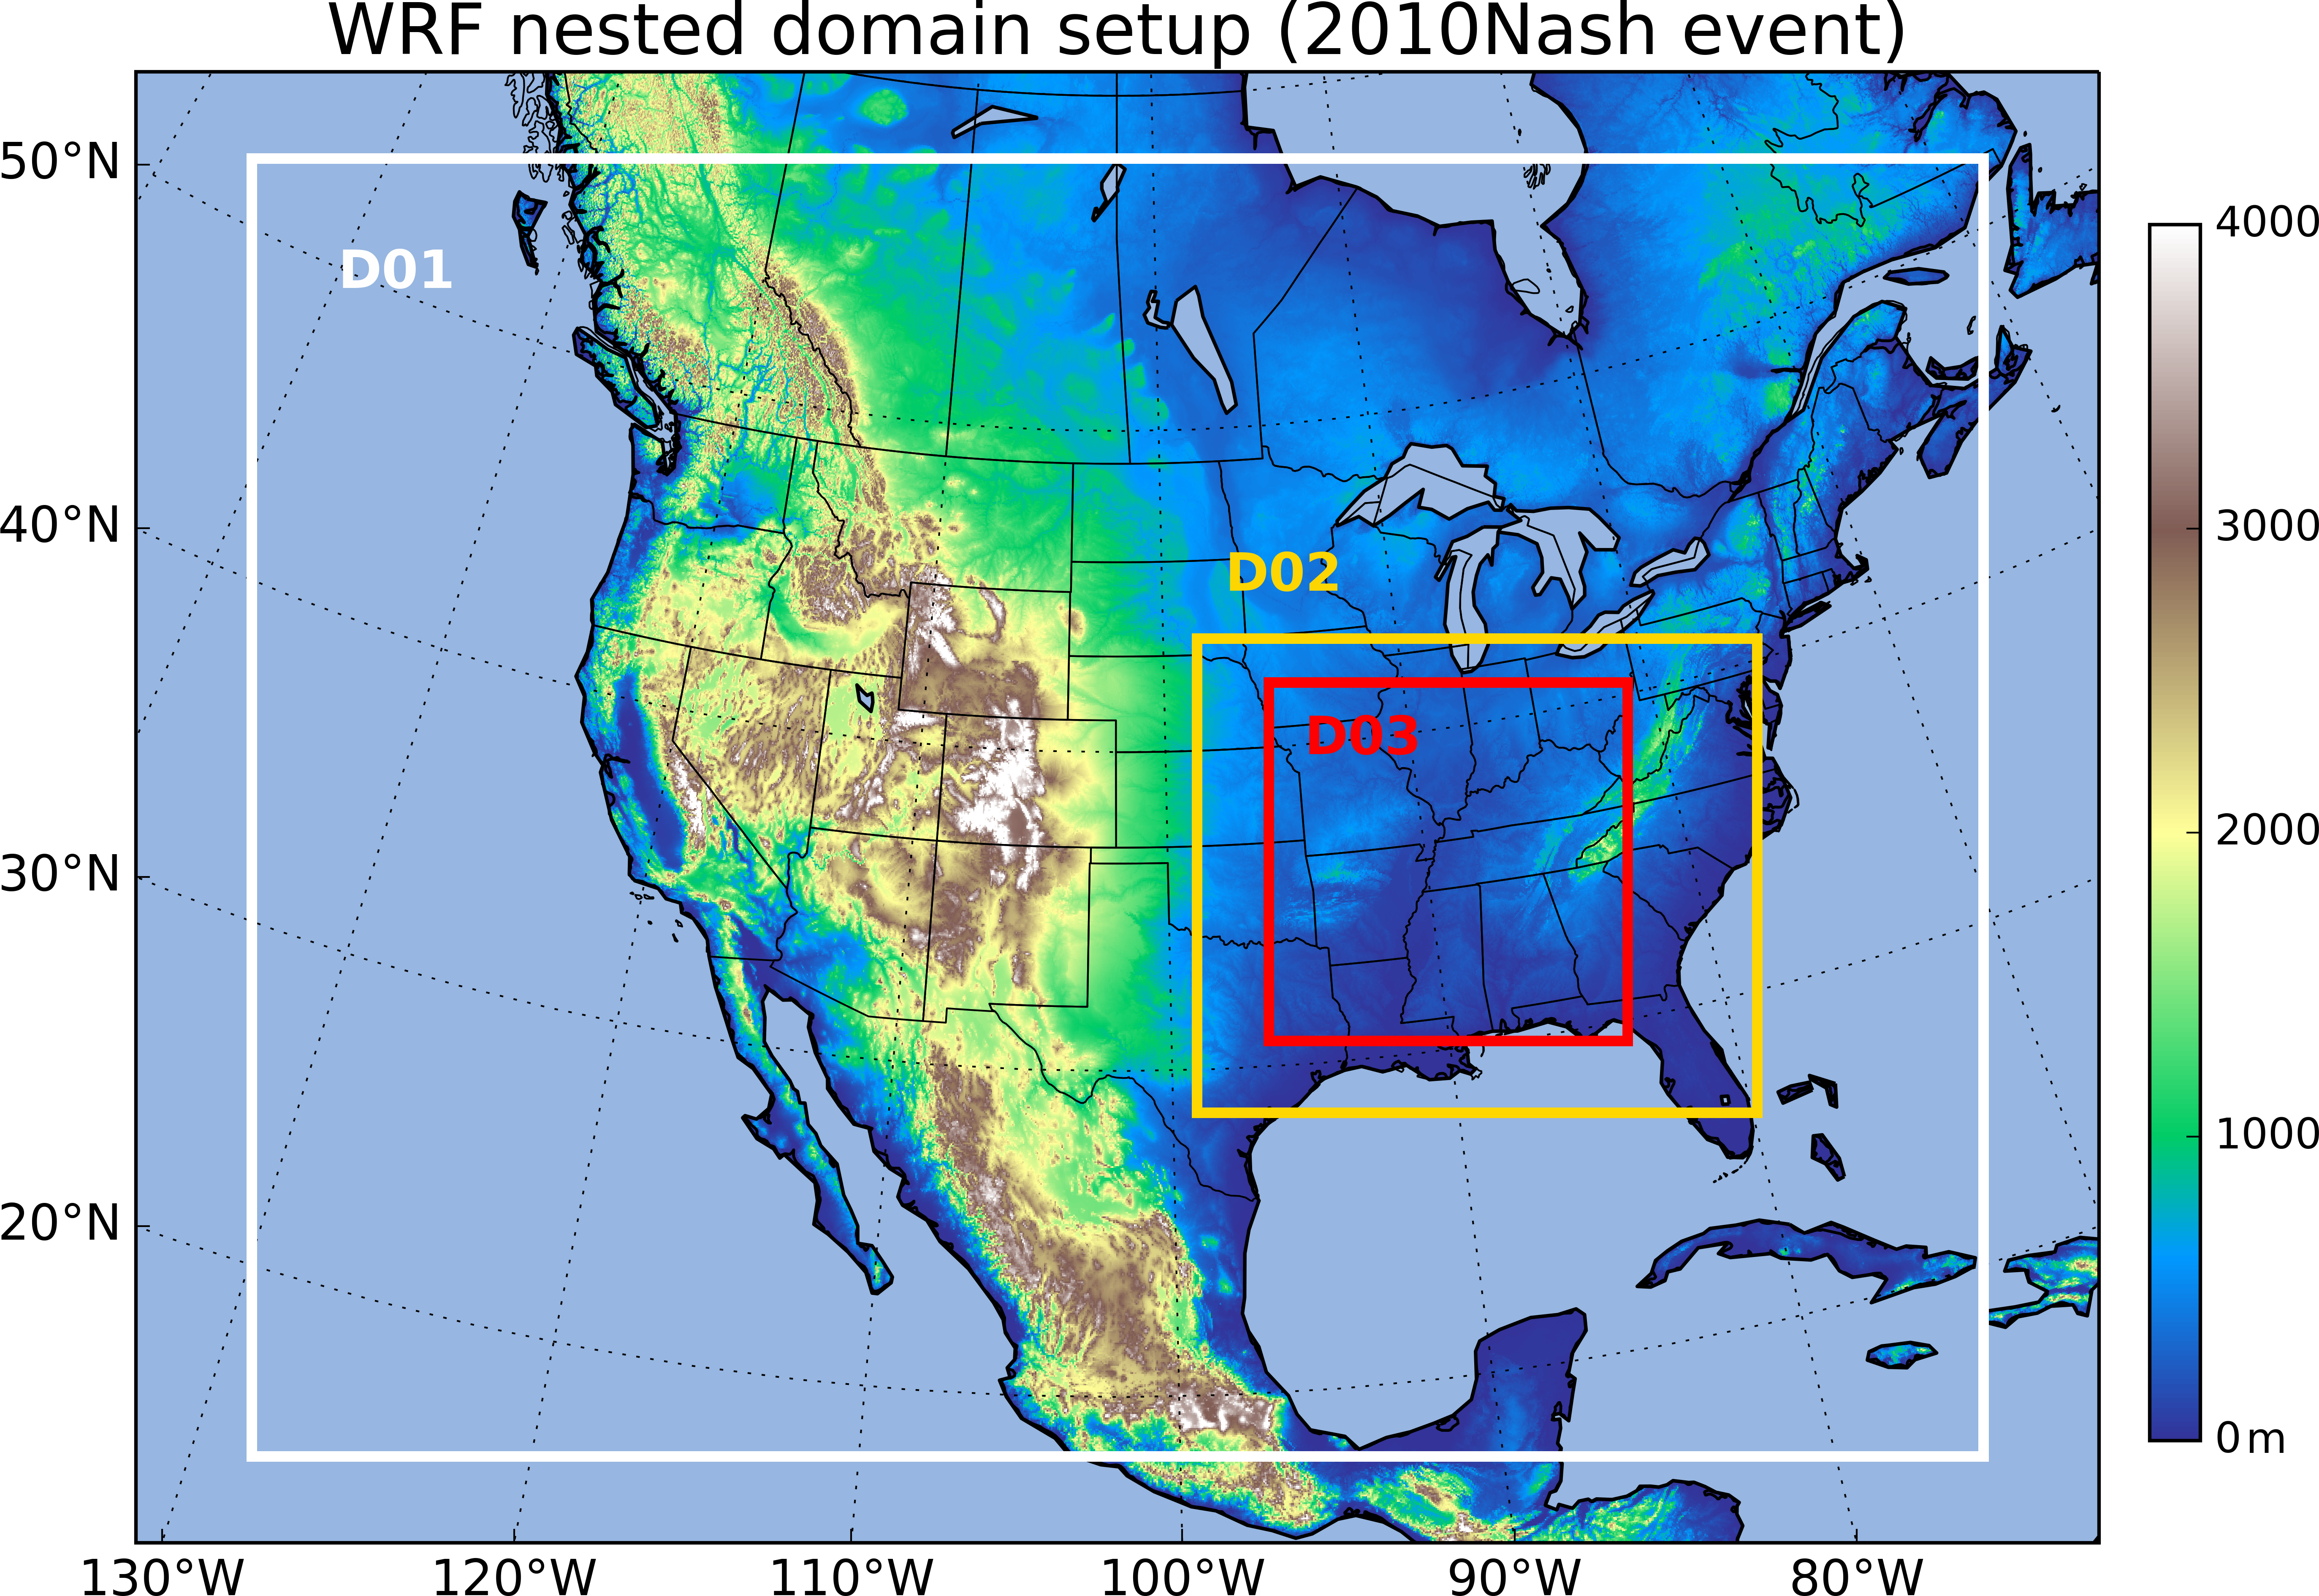
\includegraphics[width=10cm]{pics/ch5/fig3.jpg}
	\caption{Relationship among the four PMP estimates in the experiments. The left PMP estimation (p0t0m0) uses all the historical information (historical PMP); the rightmost PMP estimation uses all the future information (future PMP); the upper PMP estimation differs from the historical PMP only in the change of maximum moisture availability due to SST warming; the lower PMP estimation reflects only the changes in the moisture track of extreme storms relative to the historical PMP. From these experiments, the difference between historical and future PMP can be decomposed into: moisture change and storm efficiency change (the blue pathway); or moisture track change and atmospheric warming (the magenta pathway).}
	\label{fig:5-3}
\end{figure}

\subsection{Robust uncertainty estimation}

Previous studies suggest that a minimum of 8-10 climate models are required to make a robust estimate on the uncertainty of a climate variable [\textit{Mote et al.}, 2011]. Here we use 10 models in total to derive a robust uncertainty estimation.

First is the adjustment of the ensemble. As shown in Figure \ref{fig:5-S1} and \ref{fig:5-S2}, the mean of maximum 3-day precipitation and the moisture maximization ratio are almost the same between the 5-model ensemble and the 10-model ensemble. Therefore, the ensemble mean estimation of PMP does not require adjustment.

Then the uncertainty can be estimated for each step of the PMP estimation, following an approach proposed in \textit{Micovic et al.} [2015]. By dividing the total uncertainty into uncertainty within the maximum 3-day precipitation and within the maximization ratio, the variation of the 10-model ensemble PMP, i.e. $Var10(PMP)$, can be approximated using equation \ref{eq:5-4}.

\begin{equation}
	Var10(PMP) = Var5(PMP) \times \frac{{Var10(max\_3day\_P)}}{{Var5(max\_3day\_P)}} \times \frac{{Var10(maximization\_ratio)}}{{Var5(maximization\_ratio)}}
	\label{eq:5-4}
\end{equation}

Where $Var5(X)$ is the standard deviation of $X$ based on the 5-model ensemble, and $Var10(X)$ is the standard deviation of $X$ based on the 10-model ensemble.

The moisture maximization ratio is taken as the average ratio in the ocean region within $15^{\circ}$N-$55^{\circ}$N and from $180^{\circ}$W to the US west coast. In estimating the maximization ratio, it is necessary to define an “event $PW$”. This event $PW$ is estimated using the $X\%$ exceedance frequency $SST$. Since most of the extreme precipitation events in the PNW happen in winter, we vary X between 0 to 50, and it turns out that the maximum $Var10(maximization ration)/Var5(maximization)$ is about 1.1 (Figure \ref{fig:5-S3}). Therefore, 110\% is used in equation \ref{eq:5-4} to extend the uncertainty in the maximization ratio obtained from the 5-model ensemble.

\section{Results}

\subsection{AR simulation skill in CMIP5}

\begin{figure}[htbp]
	\centering
	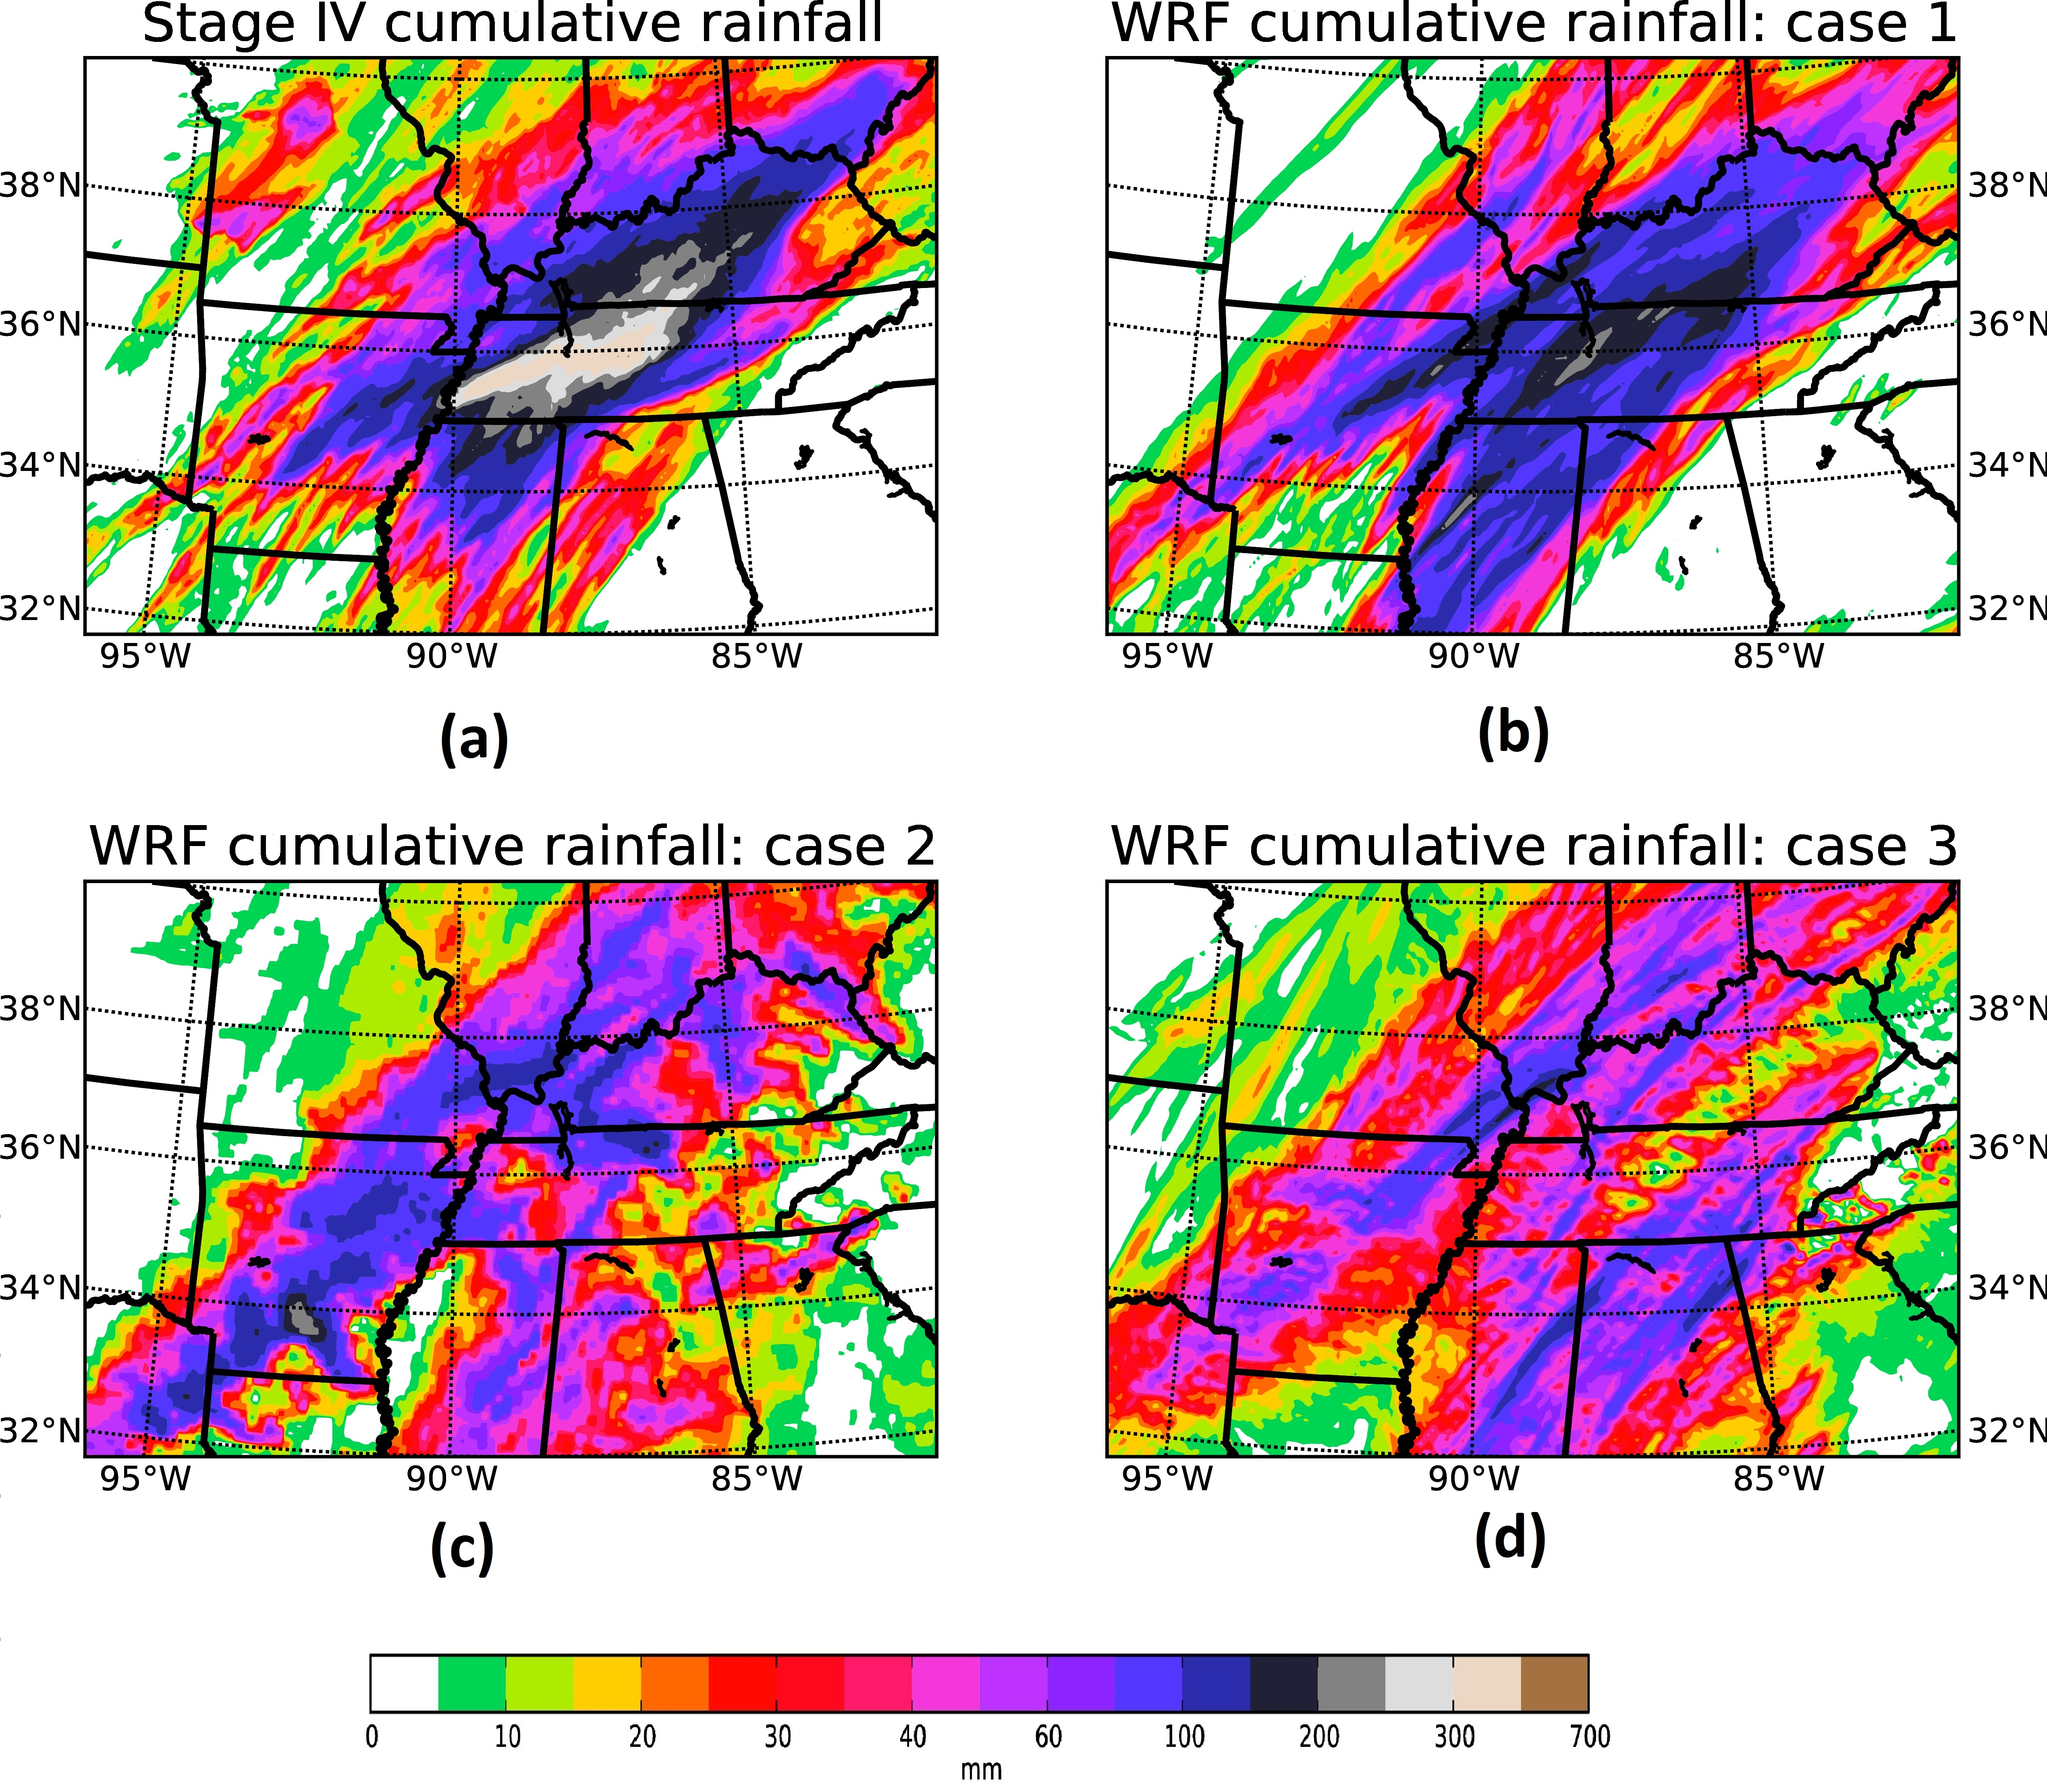
\includegraphics[width=10cm]{pics/ch5/fig4.jpg}
	\caption{Comparison of CMIP5 simulated atmospheric river (AR) climatology defined as the number of AR days over PNW with reanalysis data. Black line shows the mean of 4 reanalysis products (CFSR, ERA-Interim, MERRA and NCEP1), red lines show the AR frequency in 5 CMIP5 models used for PMP estimation (ACCESS1-0, CMCC-CM, CNRM-CM5, GFDL-ESM2G and MPI-ESM-LR), and blue lines are the AR statistics from 5 additional CMIP5 models for uncertainty estimation (ACCESS1-3, CanESM2, HadGEM2-CC, HadGEM2-ES and MIROC5). Grey lines show the AR statistics from all the 22 evaluated CMIP5 models. Data is taken from \textit{Gao et al.} [2015].}
	\label{fig:5-4}
\end{figure}

Extreme storms in the PNW region are strongly influenced by AR events [\textit{Leung and Qian}, 2009]. Consistently, ARs accounted for most of the flooding events in Washington State [\textit{Neiman et al.}, 2011]. Thus it is important that the climate models used in the PMP estimation skillfully simulate the AR climatology. Figure \ref{fig:5-4} shows the simulated AR days over the PNW from 24 CMIP5 models as gray lines, as well as the mean of four reanalysis products (CFSR, ERA-Interim, MERRA, and NCEP1) as black line, as analyzed by \textit{Gao et al.} [2015]. Here AR days refer to the number of days with an AR detected along the PNW coast ($40^{\circ}$N-$50^{\circ}$N). It is clear that ARs make landfall in the PNW coast more frequently in fall and winter. All 24 CMIP5 models have realistic seasonality, but some of them fail to capture the increased AR days from fall to winter. Based on this evaluation, five CMIP5 models that can best capture the AR days climatology (red lines) are selected for PMP estimations in this study. The blue lines show the performance of the five additional models for PMP uncertainty check, and most of them also exhibit the similar trend of AR days in autumn and winter.

\subsection{Historical PMP estimation}

\begin{figure}[htbp]
	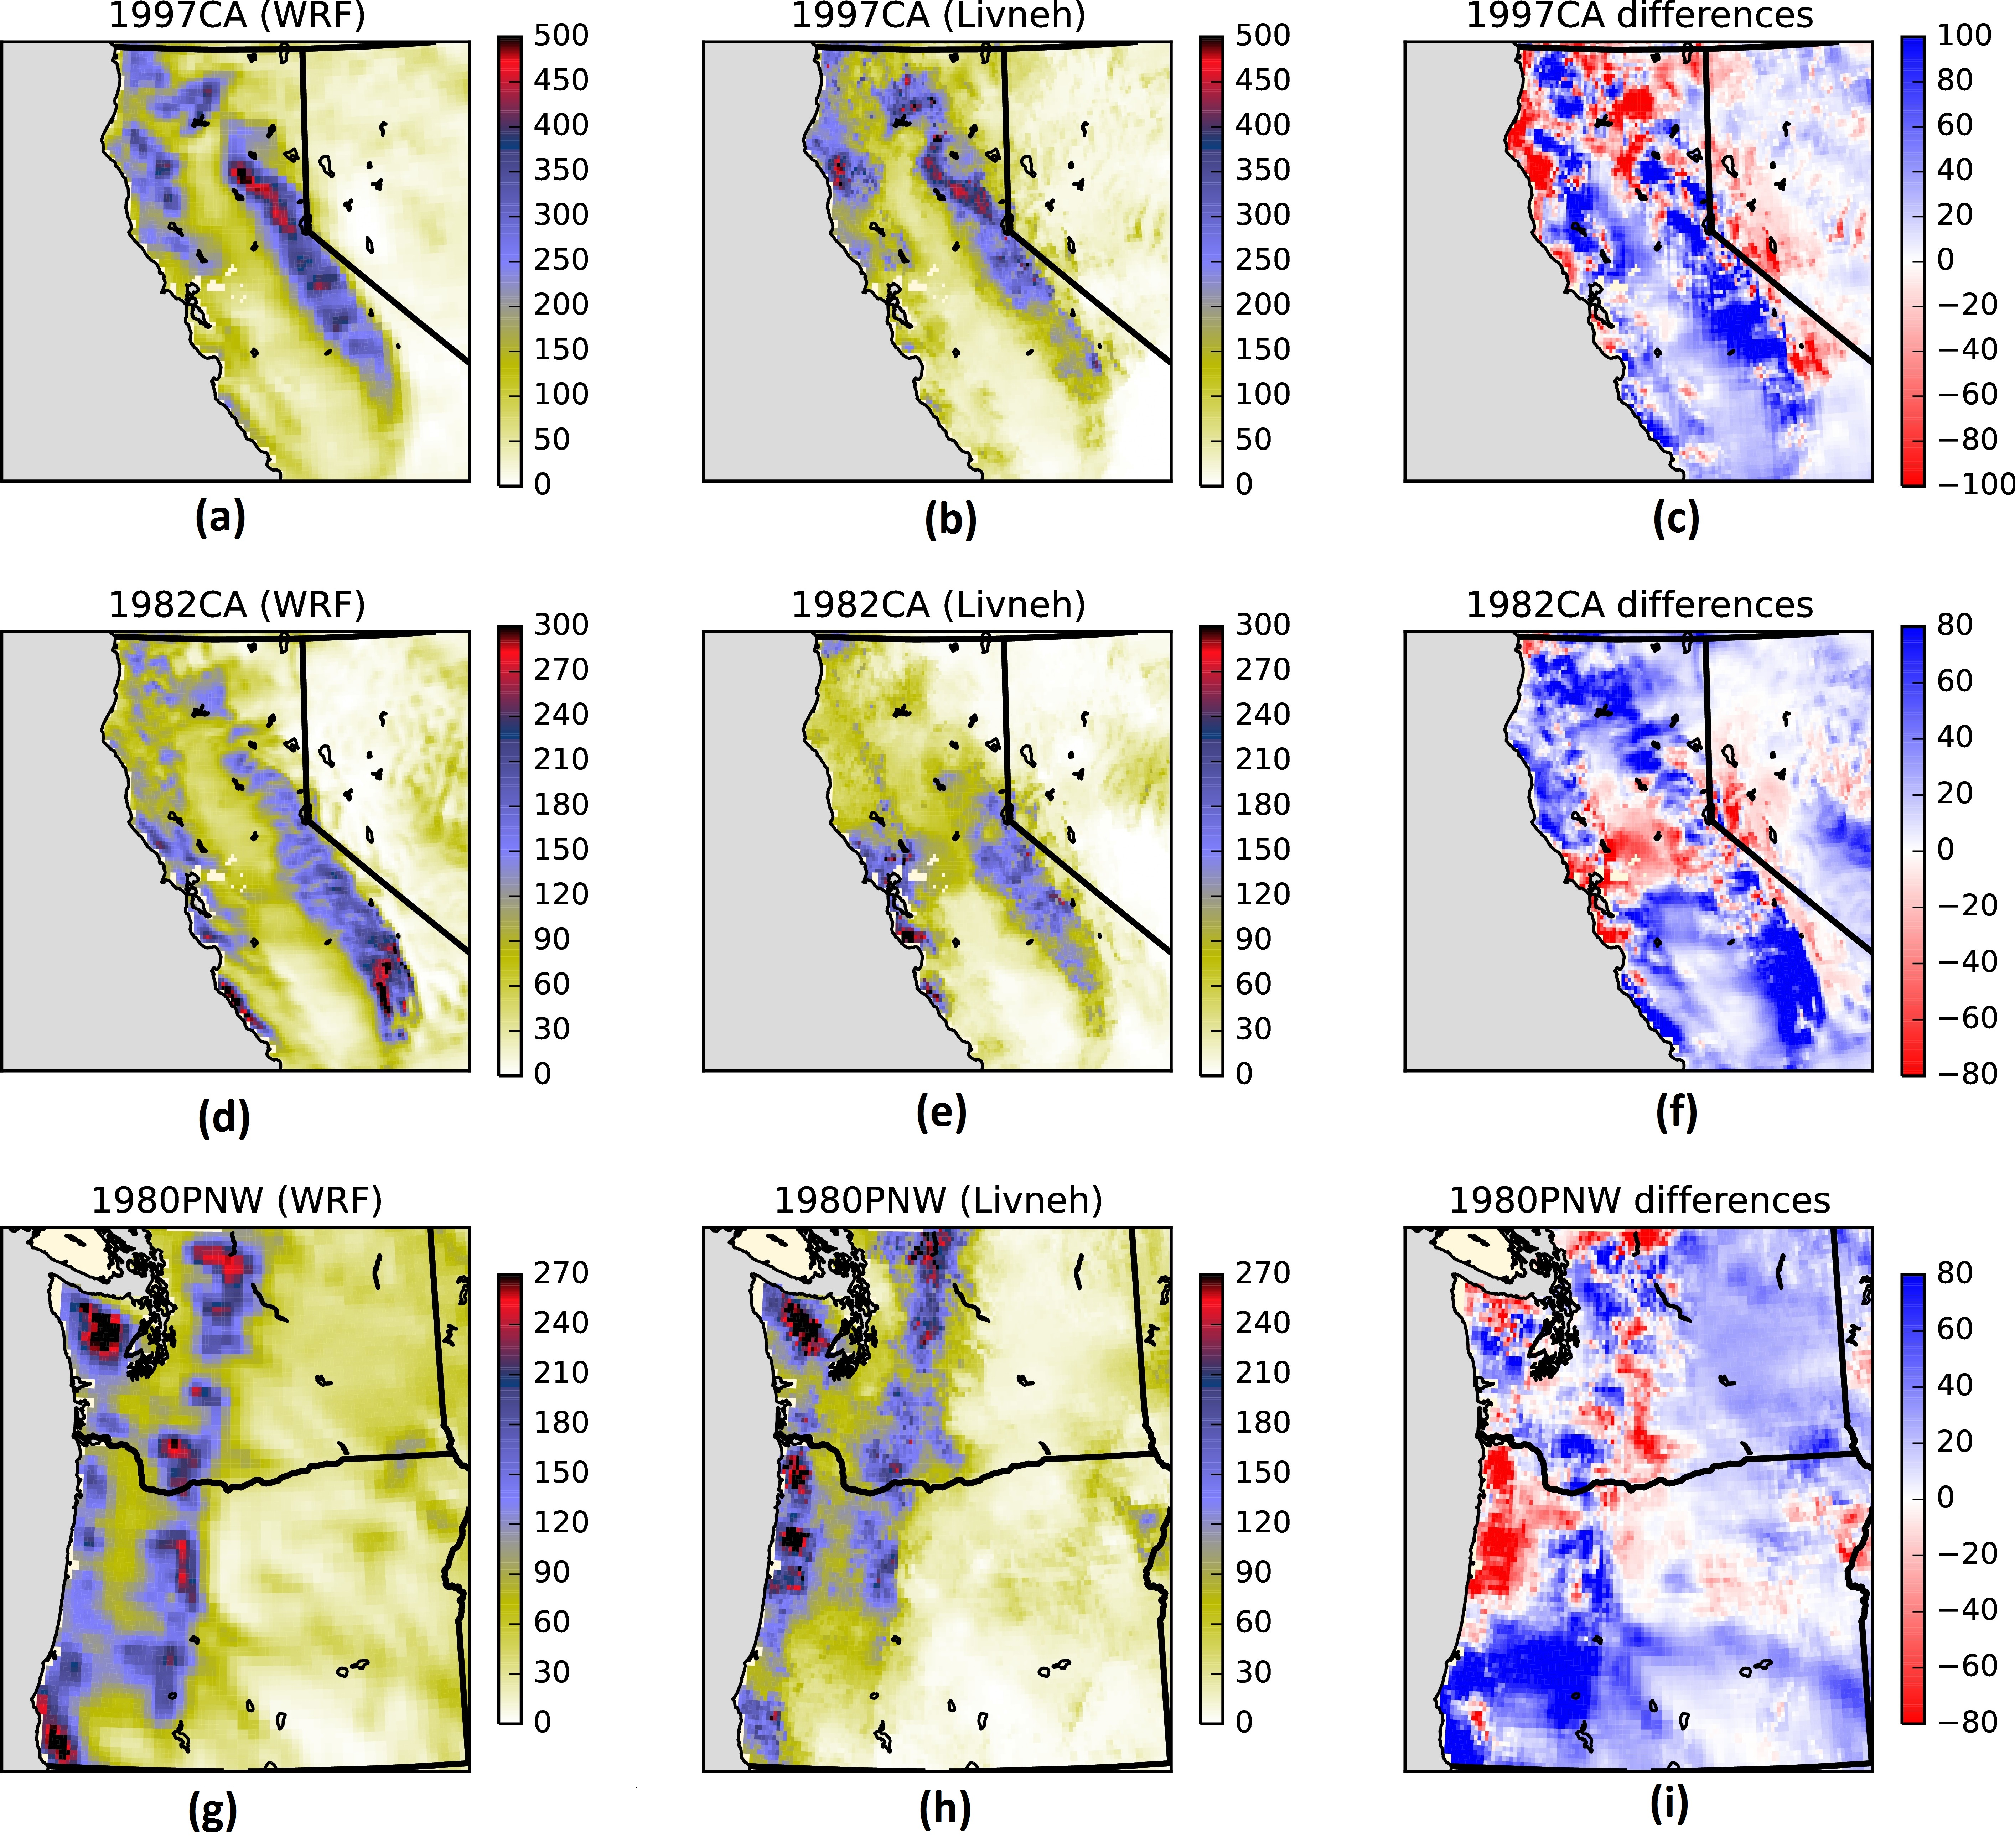
\includegraphics[width=\linewidth]{pics/ch5/fig5.jpg}
	\caption{Locations of the 43 PMP estimation sites in the HydroMeteorologial Report (HMR) 57. Red dots denote the locations of dams/reservoirs, and blue areas are the upstream watersheds of these sites. The background is the Hydrological Unit (HU) watersheds in the PNW region. Upstream watersheds are derived using the river network database in \textit{Wu et al.} [2012].}
	\label{fig:5-5}
\end{figure}

Since we combined the traditional engineering practice with climate model data, it is useful to compare the hybrid PMP estimation with the established PMP values to determine a common baseline. Figure \ref{fig:5-5} shows the sites of the established PMP values in HMR 57 (red dots), as well as their upstream watersheds as derived from river network database [\textit{Wu et al.}, 2012]. Figure \ref{fig:5-6} compares the HMR PMP values to the hybrid PMP values estimated using data from each CMIP5 model (5a to 5e), as well as the multi-model ensemble (MME) mean historical estimation based on the five models (5f).

\begin{figure}[htbp]
	\includegraphics[width=\linewidth]{pics/ch5/fig6.jpg}
	\caption{Evaluation of the hybrid historical PMP estimation against established values in HMR. The HMR PMPs are taken from basins shown as the red dots in Figure \ref{fig:5-1} and compared to the hybrid estimation. Panels (a)-(e) are the PMP estimates from individual CMIP5 models, and panel (f) shows the ensemble mean and standard deviation of PMP estimation in the basins. Blue lines are the regression between HMR PMP and hybrid PMPs.}
	\label{fig:5-6}
\end{figure}

Regarding the PMP values, the performance among the five models varies, from heavy underestimation in CMCC-CM to slight overestimation in MPI-ESM-LR. The five models can be classified into 3 groups: 1) CMCC-CM, which underestimates PMPs in all evaluation watersheds; 2) CNRM-CM5, ACCESS1-0 and GFDL-ESM2G, which provide consistent estimates as HMR, with slightly underestimated PMPs in certain basins; 3) MPI-ESM-LR, which slightly overestimates PMPs than HMR. Despite this variation, all 5 models correctly reproduce the spatial heterogeneity and the magnitude of PMP with the lowest correlation coefficient of 0.67, which is acceptable given the range of available HMR PMPs (between 150mm and 900mm) and the varying sizes of the upstream watersheds (between 9 and 10,900 mile2) in the domain. The MME mean still tends to underestimate PMPs, but the HMR values fall within the envelope of the MME range in most watersheds (panel \ref{fig:5-5}f). The variation of MME increases as the PMPs become larger, which suggests increased variations in the extreme precipitation simulation in the models. It is also interesting to see that the simulated PMP does not always benefit from the use of finer resolution climate model data; with the finest atmospheric grid size among the five models, CMCC-CM produces the most biased results. Since we used the LOCA downscaled precipitation, biases in the GCM precipitation are inherently removed so the effects of model resolution on precipitation are minimized. Differences in the hybrid PMP skill among the models are likely related to model biases in the moisture tracks and SST relative to the observations, which are not expected to have a simple relationship with the model grid sizes.

\begin{figure}[htbp]
	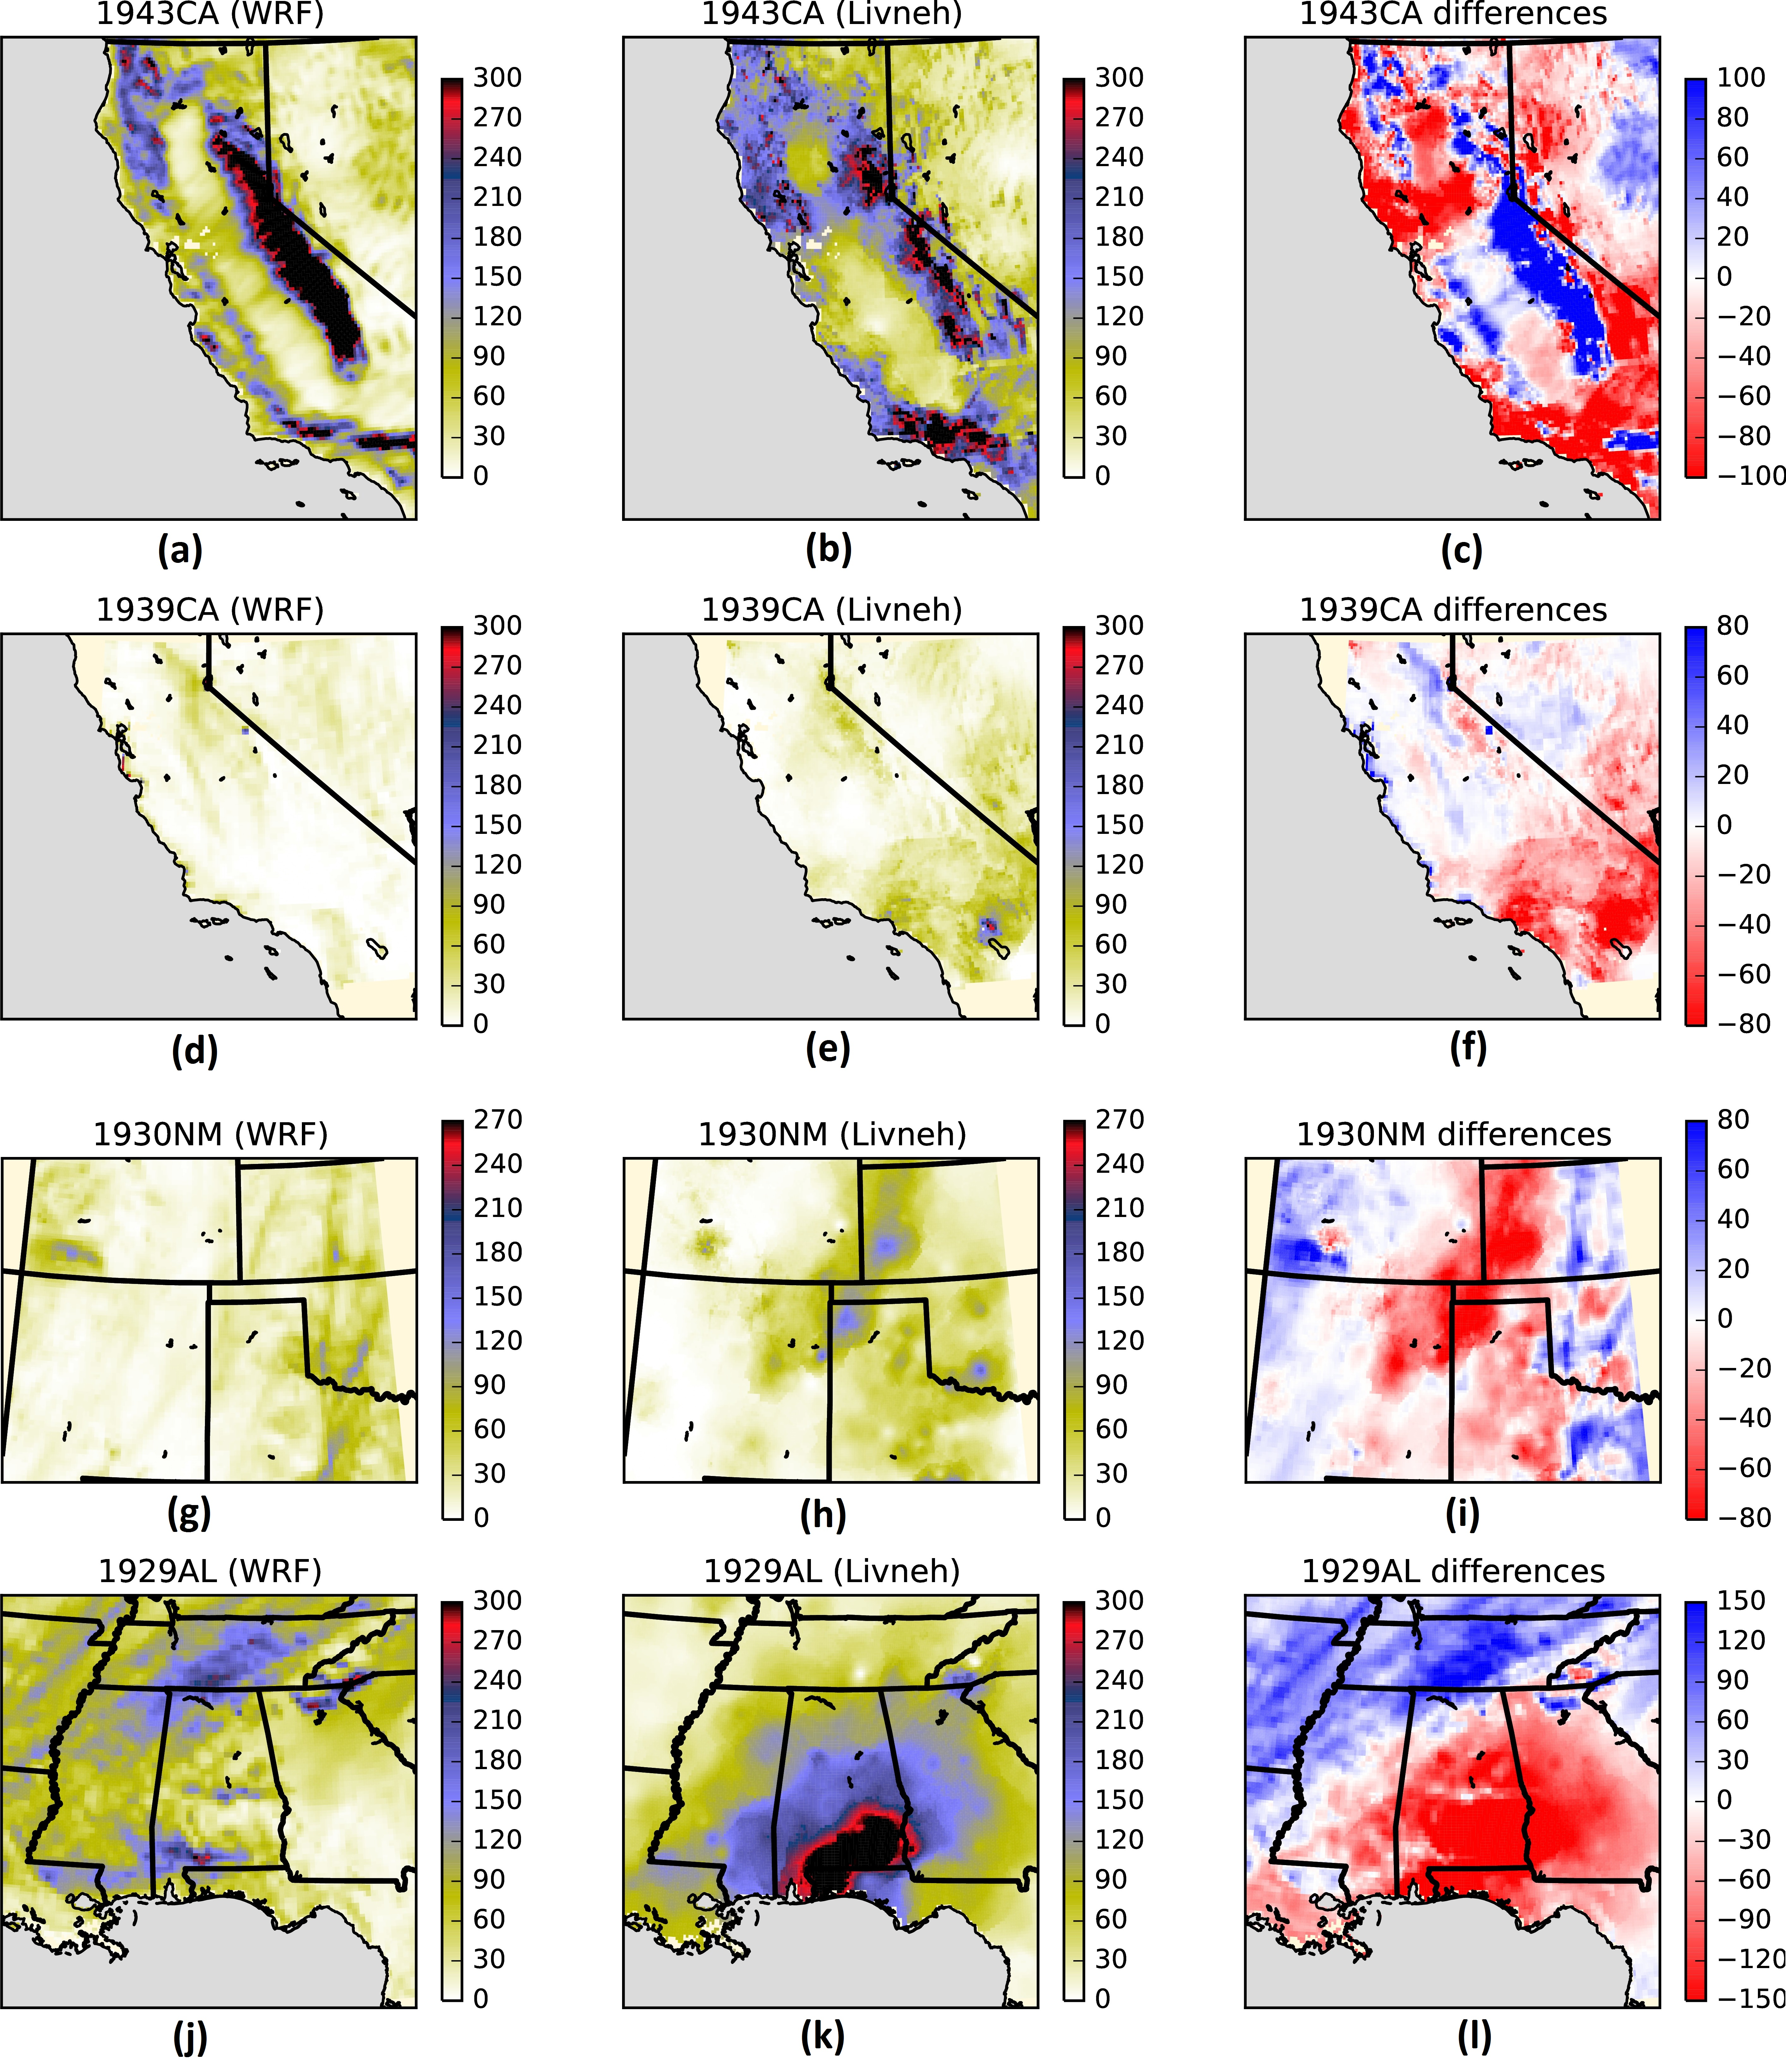
\includegraphics[width=\linewidth]{pics/ch5/fig7.jpg}
	\caption{Hybrid PMP estimation from 5 selected CMIP5 models. Panel (a) is the multi-model ensemble mean PMP estimation using CMIP5 data for 1970-2016, and (b) shows the standard deviation (as percentage of the mean) among 5 models. Panels (c)-(g) are the PMP estimations from 5 individual models.}
	\label{fig:5-7}
\end{figure}

Figure \ref{fig:5-7} presents the geographic distribution of the hybrid PMP estimation. All 5 models show much higher PMP in the coastal region and a dramatic drop east of the Cascade Range. The PMP increases further east in the northern Rocky mountain range. This spatial pattern reflects the spatial variations of storm efficiency as influenced by topography and the spatial variations of the moisture source regions. The spatial pattern of PMP is most significant in CNRM-CM5 and GFDL-ESM2G, and least significant in CMCC-CM, which is reflected in the regression in Figure \ref{fig:5-6}.  The uncertainty (i.e. standard deviation) of the hybrid PMP does not display strong spatial patterns (panel \ref{fig:5-7}b), and overall the standard deviation is about 20\% of the MME mean. However, larger disagreement among different models is found in the southeast region of PNW, but PMP values are very small in that region.

\subsection{PMP change with climate warming}

\subsubsection{Total change of PMP}

\begin{figure}[htbp]
	\includegraphics[width=\linewidth]{pics/ch5/fig8.jpg}
	\caption{Changes of PMP by 2099 compared to PMP by 2016. Panel (a) shows the amount of change in mm, and panel (b) shows the change as percentage of historical PMP (1970-2016).}
	\label{fig:5-8}
\end{figure}

Figure \ref{fig:5-8} compares the PMP estimations between the historical period (1970-2016) and future period (2050-2099), from the two experiments p0t0m0 and p1t1m1, respectively. PMP increases in all PNW watersheds by up to 500mm or 100\% (Figure \ref{fig:5-8}). The absolute change in PMP is largest in watersheds in the coastal range and Cascades range that already experiences more severe precipitation climatologically (panel \ref{fig:5-7}a). Percentage wise, the increase in PMP is more homogeneous across the watersheds, with an overall increase of about 50\%.

\begin{figure}[htbp]
	\centering
	\includegraphics[width=10cm]{pics/ch5/fig9.jpg}
	\caption{Historical (by 2016) and future (by 2099) PMP in PNW from CMIP5 ensemble estimation. Panel (a) shows the uncertainty from 5-model estimation, and (b) shows the results from 10-model estimation. Black lines are the historical multi-model ensemble (MME) historical mean PMP, and blue lines are the future mean PMP. Green and magenta ranges are the standard deviation in the MME estimation for historical and future period, respectively. All the data are normalized by the historical MME mean values (left y-axis). After the normalization, all historical MME mean is equal to one (black line). The actual values of the historical MME mean are shown in the red line (right y-axis). The x-axis shows the 220 HU8 basins, which are arranged by their historical MME mean PMP with decreasing PMP values from left to right.}
	\label{fig:5-9}
\end{figure}

To appreciate the significance of the PMP increase in the future, Figure \ref{fig:5-9} shows the 220 hydrological units in the domain along the x-axis, arranged by their historical MME mean PMP from high values to low values (red line). The PMP values indicated by the y-axis on the left-hand side of the figure are all normalized by the historical 5-model MME mean PMP (which is the same as the 10-model MME mean, as demonstrated in section 2.5), and the green envelope shows the range (defined as standard deviation) of MME estimates in the historical period. The blue line and magenta envelope show the MME mean and the range (defined as standard deviation) of PMP in the future. Panel 9a shows the uncertainty from the 5-model ensemble, and 9b shows the 10-model ensemble results. For most watersheds, the future MME mean PMP is well outside the ensemble range of the historical MME, and vice versa, so the increase depicted in Figure \ref{fig:5-7} is significant. On average, the future MME mean PMP has an increase of about 50\% over the historical MME mean across the domain, but in several watersheds the future PMP can increase by as high as 100\% of the historical PMP. There is a tendency for the relative uncertainty (range) to increase from wet watersheds (basins on the left side of the x-axis) to the dry watersheds (basins on the right side of the x-axis). In absolute terms, the uncertainty (range) still decreases from wet watersheds to the dry watersheds.

\subsubsection{Sensitivity of PMP to climate factors}

\begin{figure}[htbp]
	\includegraphics[width=\linewidth]{pics/ch5/fig10.png}
	\caption{Changes of PMP corresponding to each contributing factor. Panel (a) breaks down the total change into changes due to moisture availability and changes due to storm efficiency change. Panel (b) breaks down the total changes into changes due to storm track shift and changes due to warming.}
	\label{fig:5-10}
\end{figure}

Two sensitivity experiments (p0t0m1 and p10t10m10) were designed to examine the impact of individual climate change factor on the PMP change. As described in the method section, the total change of PMP can be either broken into available moisture change and storm efficiency change, or storm track change (dynamical effect) and warming (thermodynamical effect). Figure \ref{fig:5-10} shows the relative contribution of these factors. From panel \ref{fig:5-10}a, the increase of maximum moisture availability due to warming explains 92\% of the total increase in PMP, while the storm efficiency increase is responsible for the rest or 8\% of the increase. As illustrated in panel \ref{fig:5-10}a, changes in storm efficiency lead to a decrease of PMP in some basins. This negative contribution of storm efficiency change is consistent with the earlier finding that storm efficiency would decrease in a warming climate due to increase in atmospheric stability [\textit{Pauluis}, 2015]. However, if the increase of moisture can offset the decrease in the storm efficiency, the future PMP will still increase. Panel \ref{fig:5-10}b shows that atmospheric warming accounts for over 132\% of the total PMP change, while moisture track shift has a contribution of -32\% to the PMP increase. The latter result is consistent with \textit{Warner et al.} [2015] and\textit{ Gao et al.} [2015], who found that changes in AR frequency and moisture transport in the North Pacific ARs are dominated by changes in atmospheric moisture associated with warming in the future. Also, \textit{Gao et al.} [2015] found that changes in moisture pathways counter the increase in AR days due to warming, and our results also show opposite contributions of moisture track change and warming to PMP increase in the future.

\begin{figure}[htbp]
	\includegraphics[width=\linewidth]{pics/ch5/fig11.jpg}
	\caption{Contribution of different factors to the future change of PMP in the PNW. Panel (a) and (b) show the relative contribution (in percentage of total change of PMP) from increased moisture availability and increase storm efficiency. Panel (c) and (d) shows the relative contribution from shifted storm track and atmospheric warming.}
	\label{fig:5-11}
\end{figure}

Figure \ref{fig:5-11} shows the spatial distribution of the relative contributions of the four factors to PMP changes in the future. Both moisture availability and storm efficiency have a domain-wide impact, although moisture is more dominant. Comparing panel \ref{fig:5-8}b with panels \ref{fig:5-11}a and \ref{fig:5-11}b, watersheds with an above-average percentage increase in PMP tend to be where storm efficiency plays positive roles in PMP changes. Notably, watersheds showing increased (decreased) contribution from storm efficiency are mostly located on the lee (windward) side of mountain ranges. This coincides with the findings that orographic precipitation tends to shift downwind in response to surface warming due to an upward shift of condensation with warming [\textit{Siler and Roe}, 2014]. Since LOCA provides spatial downscaling of precipitation through the use of historical analog, it can capture some effects of orographic adjustment but the extent to which it can represent changes in orographic precipitation in response to dynamical and thermodynamical changes in the atmosphere is not clear. Hence the mechanisms for the changes in precipitation spatial distribution deserve further investigation in the future. Panel \ref{fig:5-11}c and 11d show the partitioning of PMP changes contributed by storm track shift and warming, respectively. Warming plays a clear dominant role, and storm track shift results in noticeable positive changes in only a small number of watersheds. Interestingly, watersheds that have larger contributions from moisture track shift (panel \ref{fig:5-11}c) tend to also exhibit larger contributions from storm efficiency (panel \ref{fig:5-11}b). A possible explanation for these coincidental changes is that wind direction changes related to moisture track shift have an influence on orographically induced upward and downward motions, and hence storm efficiency. For example, several of the watersheds with notable positive contributions from moisture track shift and storm efficiency change are located on the lee side of the Cascade Range where changes from westerly to southwesterly winds may increase storm efficiency.

\section{Discussion}

\subsection{Factors affecting PMP estimation quality}

As can be seen from equation \ref{eq:5-1}, PMP based on the hybrid method is sensitive to the quality of the simulated precipitation and precipitable water and the SST field. Figures \ref{fig:5-6} and \ref{fig:5-7} show differing capabilities of CMIP5 models in capturing PMP in PNW. In this study, the differences in performance of the CMIP5 models in simulating precipitation may be reduced by the LOCA downscaling process, which includes bias correction and spatial downscaling. Using raw CMIP5 output could result in very different PMP estimation, so potentially a larger ensemble of GCMs should be used to characterize uncertainty if raw CMIP5 data were used.

SST data used in the PW estimation is obtained via back trajectory, so the first concern is the resolution of the climate models. Panels \ref{fig:5-6}(a-e) are arranged by the atmospheric model resolution, from $0.75^{\circ}$ in CMCC-CM to $2^{\circ}$ in GFDL-ESM2G. PMP estimation in CMCC-CM does not benefit from the higher resolution of atmospheric models, while GFDL-ESM2G is the within top two of the five models. Therefore, climate model resolution may not positively affect the PMP estimation results. This may be particularly true as one may expect larger impacts of model resolution on precipitation, but such impacts have been minimized by using statistically downscaled precipitation. On the other hand, previous studies showed that a minimum spatial resolution of about 12km is needed to fully resolve the spatial characteristics of cold season extreme precipitation in mountainous regions, so the impact of model resolution may be more significant as we approach a much finer resolution [\textit{Prein et al.}, 2013].

Precipitation and SST also have a direct impact on the PMP estimation in equation \ref{eq:5-1}. Since statistical downscaling method takes the same ground observation as a reference, the downscaled precipitation among climate models is made close to each other (via similarities to the reference data). The CMIP5 SST data are evaluated using NOAA’s Optimum Interpolation SST dataset (OISST, \textit{Reynolds et al.} [2007]; \textit{Banzon et al.} [2016]) for the overlapping period of 1982-2016, and the results are summarized in Table 3. The mean and variation are similar across the five models, but the construction of the maximum SST differs much more. It is important to point out that most of the extreme precipitation events in PNW occur in winter when SST is relatively cooler, so the SST during winter storms should be more characteristic of the PMP biases. Indeed, the bias (RMSE) of the constructed maximum SST also shares a lot of similarities with Figure \ref{fig:5-6}, where CMCC-CM has the largest bias in the estimated PMP, and CNRM-CM5 has the least biases. This can be explained by the relationship between SST and PW used in practice [\textit{World Meteorological Organization (WMO)}, 1986]: PW follows an approximately exponential relationship to SST, which heavily amplifies small biases in the maximum SST when SST is high. This, in turn, affects the maximization ratio, and therefore the final PMP estimation. As shown in panel \ref{fig:5-10}a, given all other factors (precipitation, representative SST of events) unaltered, the increase of maximum SST alone is responsible for 92\% of the future PMP increase. This suggests that the impact of warming on PMP increase is most likely a response to the increases in SST, which increases atmospheric moisture availability.

\begin{table}[htbp]
	\centering
	\caption{Evaluation of CMIP5 simulated daily SST}
	\begin{threeparttable}
		\begin{tabular}{ccccccc}
			\hline
			\multirow{2}{*}{Model} & \multicolumn{2}{c}{mean} & \multicolumn{2}{c}{std} & \multicolumn{2}{c}{max} \\
			\cline{2-7}
			 & corr  & RMSE (K)  & corr  & RMSE(K)  & corr & RMSE(K) \\
			\hline
			CMCC-CM & 0.993 & 1.367 & 0.907 & 0.464 & 0.980 & 2.716\\
			CNRM-CM5 & 0.995 & 0.862 & 0.967 & 0.498 & 0.982 & 1.191\\
			ACCESS1.0 & 0.995 & 0.922 & 0.909 & 0.482 & 0.960 & 2.132\\
			MPI-ESM-LR & 0.993 & 1.171 & 0.918 & 0.438 & 0.980 & 2.101\\
			GFDL-ESM2G & 0.994 & 1.538 & 0.901 & 0.617 & 0.971 & 1.620\\
			\hline
		\end{tabular}
		\begin{tablenotes}
			\small
			\item The evaluation is done in the 1982-2016 duration, with NOAA’s OISST as reference.
		\end{tablenotes}
	\end{threeparttable}
	\label{table:5-3}
\end{table}


\subsection{Evaluation of the performance of climate model output}

\begin{figure}[htbp]
	\includegraphics[width=\linewidth]{pics/ch5/fig12.jpg}
	\caption{Historical 3-day PMP estimation from alternative approaches. Panel (a) estimates PMP using the hybrid approach in this study, but with the 1982-2013 Livneh precipitation observation, ERA-Interim reanalysis winds, and SST observation. Panel (b) is similar to (a), but with SST observation replaced by the precipitable water in ERA-Interim. Panel (c) estimates PMP using the approach proposed by \textit{Rouhani and Leconte} [2016] and the 2001-2012 4-km WRF simulation of the continental US [\textit{Liu et al.}, 2017]. In all three panels, the x-axis shows the PMP values in HMR 57, and the y-axis shows the values from three alternative approaches.}
	\label{fig:5-12}
\end{figure}

Figure \ref{fig:5-12} shows the various experiments conducted using alternative data sources/approaches. Panel \ref{fig:5-12}a uses the same hybrid approach, but with all the data from observation (i.e., Livneh precipitation, NOAA OISST SST) and reanalysis product (i.e., 6-hr ERA-Interim wind fields). PMP is estimated using the available data during 1982-2013. This observation/reanalysis-based estimation shows better spatial correlation than the CMIP5-based estimations (Figure \ref{fig:5-6}). However, the observation/reanalysis-based estimation tends to overestimate PMP.

Panel \ref{fig:5-12}b shows a similar experiment, but with OISST replaced by PW from ERA-Interim to evaluate the impact of the SST-PW relationship [\textit{World Meteorological Organization (WMO)}, 1986] on the PMP estimation. It shows that as the SST-based PW is replaced with the reanalysis PW, the final PMP is heavily overestimated. Further investigation suggests that the reanalysis assimilated PW has a wider range (1-130mm) than the SST-derived PW (8-123mm). As most of the extreme precipitation events in the PNW region happen in winter, this leads to underestimation of the event PW, and hence, the overestimation of PMP through equation \ref{eq:5-1}.

Panel \ref{fig:5-12}c shows the PMP estimation from a different approach using high-resolution climate simulation. The precipitation and PW data are taken from the 4km WRF simulation during 2001-2012 [\textit{Liu et al.}, 2017], and the PMP estimation approach is taken from \textit{Rouhani and Leconte} [2016]. This approach leads to a more biased PMP estimation even using high-resolution dynamically downscaled data. Since the WRF simulation is driven by ERA-Interim, the difference between panels \ref{fig:5-12}a and \ref{fig:5-12}c suggests the impact of different methods as well as different data sources for the PMP estimation. It shows that back-trajectory for PW search is necessary for the PNW region, which would help to keep the PMP estimation consistent with the HMR approach.

\subsection{Impact of bias in the input data on the final PMP estimation}

\begin{figure}[htbp]
	\includegraphics[width=\linewidth]{pics/ch5/fig13.jpg}
	\caption{Evaluation of statistically downscaled maximum 3-day precipitation in the PNW region. Here the LOCA-downscaled precipitation is compared against the PRISM gridded observation [\textit{Daly et al.}, 1994] in the 1982-2016 period. Panel (a) shows the comparison at 220 Hydrological Unit (HU) watersheds in the PNW, (b)-(d) show the comparison of the coastal/windward watersheds, leeward watersheds and watersheds in the eastern part of PNW. In all these panels, the x-axis shows the HU8 watersheds arranged by PRISM maximum 3-day precipitation, and the y-axis is the maximum 3-day precipitation from PRISM (red lines) as well as the LOCA ranges in 5-model (magenta) and 10-model (green) ensembles.}
	\label{fig:5-13}
\end{figure}

The main source of bias in the hybrid approach is from the statistical downscaling of precipitation, as well as the SST data. Panel \ref{fig:5-13}a compares the LOCA downscaled maximum 3-day precipitation against the PRISM gridded observation [\textit{Daly et al.}, 1994] across the 220 HU watersheds. In general, the extreme precipitation from LOCA exhibits good agreement with observation. If we divide the study region into three subregions: coastal/windward (panel \ref{fig:5-13}b), leeward (panel \ref{fig:5-13}c), and far east of the PNW (panel \ref{fig:5-13}d), they show varied consistencies with good agreement in the windward and leeward regions but overestimation of extreme precipitation in the far-east region by LOCA. The overestimation in eastern PNW could be related to the coarse-resolution topography of that CMIP5 models that allows more moisture to be transported across the Cascade Range to produce excess precipitation in the east. Apparently the LOCA bias-correction is not able to fully account for the overestimation because bias correction mainly removes biases for the mean and variance rather than explicitly for extreme precipitation. Based on equation \ref{eq:5-1}, this would lead to a higher estimate of PMP in the east part of the PNW region.

\begin{figure}[htbp]
	\includegraphics[width=\linewidth]{pics/ch5/fig14.jpg}
	\caption{Evaluation of the non-stationarity in the LOCA downscaled precipitation. Here the LOCA data is compared against the 4-km continental US simulation for the 2001-2012 period (a) and 2071-2099 period (b). The x-axis is the Hydrological Unit (HU) watershed, arranged by WRF maximum 3-day precipitation. The y-axis shows the max 3-day precipitation in WRF (red lines), as well as the range of LOCA 5-model ensemble (magenta) and 10-model ensemble (green). 2001-2012 WRF simulation was driven by ERA-Interim reanalysis. 2091-2099 simulation was driven by modified ERA-Interim to reflect the climate in 2070-2099.}
	\label{fig:5-14}
\end{figure}

Another bias in statistically downscaling is from the stationarity assumption of bias-correction and downscaling relationship. To check how much bias this introduces to the precipitation fields, the historical and future LOCA statistics are compared against dynamical downscaling (Figure \ref{fig:5-14}). The dynamical downscaling in Figure \ref{fig:5-14} is produced by running WRF at 4-km resolution for 2001-2012 to construct historical climate, and perturbed boundary condition to construct 2070-2099 climate [\textit{Liu et al.}, 2017]. Figure \ref{fig:5-14} indicates that under future warming, LOCA produces similar results as dynamical downscaling. Therefore, the nonstationarity within the LOCA methodology is not likely a big concern here.

Statistical downscaling techniques rely on ground observation, so the downscaled precipitation would also inherit the observational uncertainty [\textit{Henn et al.}, 2016]. Since high quality downscaled data provides precipitation that closely matches the reference observation, the uncertainty in the downscaled precipitation may exhibit similar uncertainty pattern as observation. In the PNW region, the observational uncertainty is larger over the Cascade Range region. Therefore, the observation-induced uncertainty may be worth considering in this area.

\begin{figure}[htbp]
	\includegraphics[width=\linewidth]{pics/ch5/fig15.jpg}
	\caption{Evaluation of SST in the CMIP5 models. The evaluation area is the ocean area bounded between $15^{\circ}$N-$55^{\circ}$N and $180^{\circ}$W-PNW coast. Panel (a) shows the histograms of SST in this region, and (b) shows the precipitation as calculated from SST using the relationship in \textit{World Meteorological Organization (WMO)} [1986]. In both panels, black lines are the histograms from NOAA’s Optimum Interpolation SST (OISST) observation [\textit{Reynolds et al.}, 2007; \textit{Banzon et al.}, 2016], pink lines are from 5 CMIP5 models used for PMP estimation, and green lines are the 5 additional CMIP5 models for PMP uncertainty estimation.}
	\label{fig:5-15}
\end{figure}


Biases in the SST is another potential source of bias to the PMP estimation, as any bias in SST would lead to amplified bias in PW and PWM through the non-linear relationship between SST and moisture. Figure \ref{fig:5-15} compares the CMIP5 SST to the OISST observation in the 1982-2016 duration. Panel \ref{fig:5-15}a compares the histogram of SST in the ocean regions between $15^{\circ}$N-$55^{\circ}$N, and $180^{\circ}$W-west coast. All of 10 models show similar histogram as observation. Given the low spatial variation of SST, such high consistency is expected. Panel \ref{fig:5-15}b converts the SST to the PW using the relationship from \textit{World Meteorological Organization (WMO)} [1986], and the high consistency is still clear. Therefore, SST does not require extra bias corrections.

In summary, the PMP estimation in the PNW region is likely influenced by uncertainties from different sources: PMP in the eastern part of region is more affected by extra moisture penetration in the CMIP5 models, while PMP in the western part inherits more uncertainty from the observational uncertainty of precipitation. The evaluation here indicates that for the hybrid approach to work, high-quality precipitation is the top priority.

\subsection{Usability of CMIP5 output for PMP estimation}

The biggest disadvantage of directly using the CMIP5 output in PMP estimation is the coarse spatial resolution of data. This limits the models from correctly capturing mesoscale atmospheric systems such as hurricanes and local convective systems as well as orographic rainfall, so care should be taken when using those datasets. In the PNW region, most of the extreme precipitation is associated with AR events that are features of the large-scale atmospheric circulation. CMIP5 models have demonstrated their capability in capturing such systems (Figure \ref{fig:5-4}) [\textit{Lavers et al.}, 2013; \textit{Gao et al.}, 2015; \textit{Warner et al.}, 2015] so they are suitable for PMP studies in the PNW and other regions where extreme precipitation is dominated by AR events. As discussed above, the difference in climate model resolution has no significant impact on the final estimates, and SST itself has low spatial variation. Hence the coarse-resolution precipitation data are the main limitation of CMIP5 particularly for the topographically diverse region of PNW. This issue, however, can be addressed using statistically downscaled high-resolution precipitation data that are readily available for the U.S. For PMP estimation in other regions where the moisture source for extreme precipitation may be more local, high-resolution PW data may also be required. Recently developed methods such as the adaptable random forest method presented in \textit{He et al.} [2016] provide promising venues for use with the hybrid approach before higher-resolution GCM or RCM outputs are available.

\subsection{Trade-off of using climate models in PMP estimation}

Previous studies have used dynamically downscaled climate model data [\textit{Beauchamp et al.}, 2013; \textit{Rousseau et al.}, 2014; \textit{Rouhani and Leconte}, 2016; \textit{Rastogi et al.}, 2017]. Compared with these studies, our approach involves as much raw climate model output as possible, and we show that with the advance of computationally efficient techniques (such as statistical downscaling, and HYSPLIT), the raw model output can be quickly converted to ready-to-use data for the engineering communities. We demonstrate that combining the engineering practice with climate model data provides PMP estimates that are close to the ones used in the current engineering practice. This consistency provides confidence for using our PMP estimates for the future in safety evaluation. The method tested in this study inherits some familiar issues of traditional approach (mainly the linear assumption between PW and precipitation as criticized by \textit{Abbs} [1999]). However, the hybrid method represents an important intermediate step in the transition of the current engineering approach to an entirely model-based approach. Most importantly, the hybrid method facilitates comparison with the traditional approach and allows biases to be evaluated and factors contributing to the future changes in PMP to be quantified and understood. Comparison of the hybrid approach with the full model-based approaches can reveal the influence of various storm maximization approaches used in the model by controlling the input data. Through this connection, a more reliable transition to full model-based PMP can be achieved.

In this study, PMP is estimated only through local storm maximization. In HMR57, big storms are also transposed from nearby regions (of similar climatology) to circumvent the limited or missing observational records to provide a broader collection of extreme events (e.g., rain gauge at the Nashville international airport stopped working during the Nashville 2010 May epic flooding [\textit{Chen et al.}, 2017]). With climate models, long records of extreme precipitation (and other meteorological fields) are available, which (especially as an ensemble) allow us to investigate the climate signals of extreme precipitation, thus PMP in the future climate. The complete model output fields allow us to conduct more realistic estimation, e.g., by advancing back-trajectory analysis of air mass along the surface to 3-D back-trajectory as illustrated in this study. These advantages help fulfill the demands of storm transposition, as suggested by the similarities of PMPs in Figure \ref{fig:5-5}.

\subsection{How likely will the historical PMP be surpassed in the future?}

\begin{figure}[htbp]
	\includegraphics[width=\linewidth]{pics/ch5/fig16.jpg}
	\caption{Maximum 3-day precipitation as projected by CMIP5 models. The blue line is the 10-model MME mean, and the magenta envelope is the variation (defined as standard deviation) of MME. The solid black line is the 10-model MME mean of historical max 3-day precipitation, and the black dashed line is the 10-model MME mean historical PMP. All the data are normalized by the historical MME mean PMP value (left y-axis). The actual historical MME PMP is shown as the red line (right y-axis). The light green envelope is the MME range of historical PMP. The x-axis shows the 220 HU8 basins, which are arranged by their historical MME mean PMP.}
	\label{fig:5-16}
\end{figure}

Extreme precipitation is projected to change in a changing climate, but whether future storms will exceed the design standards of existing infrastructures remains a question. This is a safety issue beyond analysis of PMP changes: if the current PMP is going to be surpassed by future storms, a safety reevaluation is more urgent than that prompted by the finding that PMP will increase. Figure \ref{fig:5-16} shows the future max 3-day precipitation as a percentage of the historical MME mean PMP. The MME range of future max 3-day precipitation and historical PMP estimation is also shown in the figure. Historical PMP (black dashed line) is about 250\% of the historical max 3-day precipitation (solid black line). Future maximum 3-day precipitation is around 45\%-50\% of the historical PMP. Thus infrastructures will not encounter “PMP storms” under the future climate. Even when considering the uncertainties in both historical PMP (light green envelope) and future max 3-day precipitation (magenta envelope), the risk of future extreme precipitation exceeding the historical design standards is still very low.

It is also worth pointing out that 3-day PMP is associated with higher uncertainties than max 3-day precipitation. According to our definition in equation \ref{eq:5-1}, PMP inherits uncertainty in the max precipitation, which is then amplified by uncertainties in the moisture condition (PW and PWM). Figure \ref{fig:5-16} shows that standard deviation of maximum 3-day precipitation is only about 20\% of the MME mean, while panel \ref{fig:5-9}b indicates that the standard deviation of PMP can be as high as 40\% of the MME mean. To further reduce the uncertainty of PMP estimation, more accurate precipitation data together with related meteorological fields (PW, temperature, winds) are all needed.

\section{Conclusions}

In this study, we applied a traditional PMP estimation approach (moisture maximization) to CMIP5 model outputs and estimated PMP over the PNW region. Model outputs from five CMIP5 models were used to assess PMP by 2016 and by 2099. The major conclusions are:

1.	Combining traditional PMP estimation approach with modern climate science and model data can provide PMP estimates that are consistent with the values used in current engineering practice;

2.	In the worst climate scenario (RCP8.5), PMP in the PNW region is projected to increase by about $50\%\pm30\%$ by 2099 relative to the 2016 level. This change is significant when considering the uncertainties of PMP estimation;

3.	Most of the increase in PMP can be attributed to climate warming, which mainly affects moisture availability through the effects on SSTs. Future change of storm efficiency and storm track tend to reduce the future PMP;

4.	PMP presents larger uncertainty than extreme precipitation. Thus it is important to have high-quality data for both extreme precipitation and the related meteorological fields (3-D wind fields, temperature) for more accurate PMP estimation.

The hybrid approach presented in this paper connects the traditional PMP estimation and model-based approaches that are becoming popular recently. This study shows that selected climate model outputs are useful for PMP estimation in certain climatological regions such as the AR dominated PNW studied here, as they present similar quality as ground-based observation data after bias correction (such as the LOCA downscaling). Attributing the contributions of various processes to the PMP change in the future using the hybrid approach yielded results that are physical and consistent with previous findings regarding the effects of warming on storm efficiency and moisture tracks. This supports the physical basis of the hybrid approach through its adoption of physically and dynamically consistent climate model outputs and effective back trajectory analysis method. Future work may further take advantage of atmospheric models and global/regional climate model data to advance state-of-the-art for PMP estimation in a changing climate.

Up to this point, all the preparations that are needed for the engineering communities to switch to physics-based PMP are ready. They are summarized and briefly discussed in the next chapter.